% ettdoc.tex V2.10, 19 June 2012

\documentclass[times]{ettauth}
\usepackage[toc,page]{appendix}
\usepackage{moreverb}

\usepackage[colorlinks,bookmarksopen,bookmarksnumbered,citecolor=red,urlcolor=red]{hyperref}

\newcommand\BibTeX{{\rmfamily B\kern-.05em \textsc{i\kern-.025em b}\kern-.08em
T\kern-.1667em\lower.7ex\hbox{E}\kern-.125emX}}

\def\volumeyear{2017}

\newcommand{\eg}{e.g., }
\newcommand{\ie}{i.e., }
\usepackage[linesnumbered,ruled,vlined]{algorithm2e}
\DeclareMathOperator*{\argmin}{arg\,min}
\DeclareMathOperator*{\argmax}{arg\,max}

\usepackage{times}
%\usepackage{mathptmx}
\usepackage{mathtools}
\usepackage[draft,nomargin,marginclue,footnote,silent]{fixme}
\setcounter{tocdepth}{2} %table of contents


\theoremstyle{mytheoremstyle}
\newtheorem{theorem}{Theorem}[section]

\theoremstyle{mytheoremstyle}
\newtheorem{corollary}{Corollary}[section]

\theoremstyle{mytheoremstyle}
\newtheorem{lemma}{Lemma}[section]

\newtheorem{mydef}{Definition}

\DeclareMathOperator*{\Max}{Max}
\DeclareMathOperator*{\Min}{Min}

\newcommand{\bigO}{\ensuremath{\mathcal{O}}}% big-O notation/symbol
\usepackage{subfigure}
\usepackage{adjustbox}
\usepackage{multirow}
\usepackage{enumitem}
\usepackage{lipsum}
\setlist[itemize]{leftmargin=*}
\setlist[enumerate]{wide=\parindent}
\usepackage[referable]{threeparttablex}
\renewlist{tablenotes}{enumerate}{1}
\makeatletter
\setlist[tablenotes]{label=\tnote{\alph*},ref=\alph*,itemsep=\z@,topsep=\z@skip,partopsep=\z@skip,parsep=\z@,itemindent=\z@,labelindent=\tabcolsep,labelsep=.2em,leftmargin=*,align=left,before={\footnotesize}}
\makeatother

\usepackage{graphicx}
\usepackage{sidecap}
\usepackage{kantlipsum} %<- For dummy text
\usepackage{mwe} %<- For dummy images
\usepackage{multirow}
\usepackage{multicol}

%% Andere Packages %%%%%%%%%%%%%%%%%%%%%%%%%%%%%%%%%%%%%%%%%%
%\usepackage{a4wide} %%Kleinere Seitenränder = mehr Text pro Zeile.
\usepackage{fancyhdr} %%Fancy Kopf- und Fußzeilen
%\usepackage{longtable} %%Für Tabellen, die eine Seite überschreiten
\usepackage{lscape}
\usepackage{rotating}
%\usepackage[htt]{hyphenat} %Trennung von Typewriter-Schriften
%\usepackage{listings}
%\usepackage{pstricks-add} --> This package generates problems with booktabs (toprule, etc.)
\usepackage[autostyle]{csquotes}
\usepackage{amsmath,bm}
\usepackage{array}
% Tabellen mit Center und left
\usepackage{tabularx,colortbl} % colored table background
%\usepackage{tablefootnote}
\newcolumntype{C}[1]{>{\centering\arraybackslash}m{#1}}
\newcolumntype{R}[1]{>{\raggedleft\arraybackslash}m{#1}}
\newcolumntype{L}[1]{>{\raggedright\arraybackslash}m{#1}}
% Table spacings
\newcommand\T{\rule{0pt}{2.5ex}\rule[-1.0ex]{0pt}{0pt}}
\newcommand\B{\rule[-1.0ex]{0pt}{0pt}}


\definecolor{slightgray}{gray}{.90}
\usepackage{rotating}
\usepackage{hhline}
\usepackage{float}
\usepackage{caption}% http://ctan.org/pkg/caption
\captionsetup[table]{format=plain,labelformat=simple,labelsep=period}
%\usepackage{authblk}

\usepackage{color}

\begin{document}

%\runningheads{A.~N.~Other}{A demonstration of the \journalabb\
%class file}

\articletype{RESEARCH ARTICLE}

\title{Robust Clustering for Ad Hoc Cognitive Radio Network}
%\author[1]{Di Li\thanks{li@umic.rwth-aachen.de}}
%\author[2]{Erwin Fang\thanks{xx}}
%\author[3]{James Gross}
\author{Di Li\textsuperscript{1}\corrauth, Erwin Fang\textsuperscript{2}, James Gross\textsuperscript{3}}
%\affil[1]{RWTH Aachen University}
%\affil[2]{ETH Zurich}
%\affil[3]{KTH Royal Institute of Technology}
\address{RWTH Aachen University\textsuperscript{1}, Swisscom (Schweiz) AG\textsuperscript{2}, KTH Royal Institute of Technology\textsuperscript{3} }
%\renewcommand\Authands{ and }
%\corraddr{Communication Theory Lab
%School of Electrical Engineering, 
%KTH Royal Institute of Technology
%SE - 100 44 Stockholm\\Email: james.gross@ee.kth.se}
\corraddr{Chair of Communication and Distributed Systems
Ahornstrasse 55 - building E3
52074 Aachen
Germany
\\Email: li@umic.rwth-aachen.de}




\begin{abstract}
%Cluster structure in cognitive radio networks facilitates cooperative spectrum sensing, routing and other functionalities.
%Unlicensed channels, which are temporally available for a group of cognitive radio users in one area, consolidate the group into a cluster.
%More available unlicensed channels in a cluster make the cluster more likely to uphold against the licensed users' influence, making clusters more robust.
%This paper analyses the problem of how to form robust clusters in a cognitive radio network such that cognitive radio systems benefit from collaboration within clusters despite intense primary user activity.
%%In the process of forming clusters, every secondary user decides with whom to form a cluster, or which cluster to join.
%We give a formal description of the robust clustering problem, prove it to be NP-hard and propose both centralized and distributed solutions.
%The congestion game model is adopted to analyze the process of cluster formation, which not only contributes to the design of the distributed clustering scheme, but also provides a guarantee on the convergence to a Nash equilibrium and the convergence speed.
%%Our proposed clustering solution is versatile to fulfill some other requirements such as faster convergence and cluster size control.
%The proposed distributed clustering scheme outperforms state-of-the-art related works in terms of cluster robustness, convergence speed and overhead.
%%Besides, we prove the clustering problem is NP-hard, and also propose the centralized solution.
%Extensive simulations are presented supporting the theoretical claims.
\end{abstract}

%\keywords{class file; \LaTeXe; \emph{\journalabb}}

\maketitle
\graphicspath{
{../figures/04_clutering/}
}

\section{Introduction}
\label{intro}
Cognitive radio (CR) is a promising approach to mitigate the increasing scarcity of radio spectrum~\cite{Mitola} arising from the common practice to license radio frequencies in a de-facto exclusive manner.
In CR, licensed users can access the spectrum allocated to them at any point in time, while unlicensed users may access the spectrum when it is not utilized. 
This can be realized by so-called opportunistic spectrum access, \ie unlicensed users access the spectrum only after validating that the channel is currently unoccupied.
In the context of cognitive radio, licensed users are also called primary users (PU), while unlicensed users are often referred to as secondary users and constitute a cognitive radio network (CRN)\footnote{The terms user and node appear interchangeably in this paper. In particular, user is adopted when its networking or cognitive ability are discussed or stressed, while we refer to nodes typically in the context of the network topology.}.
For CRN, accurate spectrum sensing is critical, and the rate of false negatives, \ie the likelihood of misdetecting active primary users, needs to be minimized~\cite{Sahai_FundamentalDesignTradeoffs2006}.
It has been shown that cooperative spectrum sensing, which relies on the consensus of CR users within a certain area, can significantly decrease the rate of false negatives despite the presence of receiver noise and wireless channel fading~\cite{Jacob2012, coorperativeSensing_Akyildiz11}.
Thus, clustering of secondary nodes is regarded as a necessary condition to realize cooperative spectrum sensing~\cite{Sun07_clustering_spectrum_secsing} for opportunistic spectrum access.

Clustering is the process of logically grouping certain users in geographic proximity.
As to wireless networking in general, and in particular with respect to wireless ad-hoc, mesh or sensor networks, clustering is known to decrease the power consumption~\cite{Kawadia03},  improve routing performance~\cite{clustering_mesh_globecom2010}, and improve the network lifetime and coverage~\cite{Abbasi_survey_07}.
For cognitive radio networks, apart from improving the sensing accuracy, clustering also improves spectrum utilization among several cognitive radio networks by allowing for coordination in particular when CRNs have to vacate channels~\cite{willkomm08}, while also been known for reducing the interference between cognitive clusters~\cite{centralizedSharing80222}, and improving routing~\cite{Abbasi_survey_07}.

In CRNs, formed clusters maintain a set of unlicensed channels which are validated by every CR node in that cluster, meaning that the channel is perceived as not being occupied by a primary user.
In the following we refer to these maintained unlicensed channels as \textit{common channels} (CC).
The availability of CCs within a cluster is elementary for the cluster, \ie if no CCs are available then the corresponding cluster can not operate any longer as CCs ascertain both control and payload data transmission within the cluster.
However, due to primary user activity, over time the list of maintained CCs of a cluster varies randomly as it is generally unknown to secondary nodes when primary users appear on different licensed channels. 
Being able to maintain a sufficiently large list of CCs ensures the \textit{robustness} of the cluster despite primary user activity, i.e. it provides a longer uninterrupted operation of the cluster.

On the other hand, the larger the cluster size is, the lower is in general the set of CCs that all nodes of a cluster observe as unoccupied by primary users.
This is due to the fact that in general, secondary nodes at different spatial locations will be able to sense the activity of different primary users due to different channel characteristics. 
Thus, a trade-off arises for the formation of robust cognitive radio clusters:
On the one hand, a low number of nodes in a cluster is desirable, as it generally provides more nodes with a common observation of primary user activity on different channels, and thus leads to a larger set of CCs, ultimately increasing the robustness. 
On the other hand, a too low number of nodes in a cluster compromises the sensing accuracy, in particular if only one or two nodes are members of a cluster~\cite{Consensus_based_clustering12}.
One therefore needs to strike a balance between the \textit{size} of a cluster and the \textit{number} of common channels per cluster, to balance robustness and sensing accuracy.
Cluster size plays furthermore a role in transmit power consumption, \ie the cluster size affects the transmit power consumption under certain routing schemes~\cite{clustering_globecom11, EnergyEfficientClusteringRouting_2015}.

In this paper, we analytically study the above mentioned trade-off which we term in the following the \textit{CRN robust clustering problem}.
We show it to be an NP-hard problem under certain assumptions, and furthermore study centralized as well as distributed algorithms.
We propose an alternate metric to measure cluster robustness in contrast to previous works~\cite{Li11_ROSS} and~\cite{LIU_TMC11_2}.
We claim that cluster robustness can not be indicated merely by the average number of CCs of a cluster, but by the ability of the cluster to uphold over time despite random primary user activity.
Our proposed distributed scheme extends our previous work ROSS (Robust Spectrum Sharing)~\cite{Li11_ROSS} by additionally incorporating control over the size of a cluster.
Throughout this paper, we call these newly proposed distributed schemes \textit{variants of ROSS}.
%
%
The rest of the paper is organized as follows:
In Section~\ref{related_work}, we review related work in particular with respect to clustering techniques in CRN.
We also discuss in more detail the relation between the contribution in this paper and our previous work in~\cite{Li11_ROSS}.
Our system model as well as the problem statement with respect to the robust clustering problem are presented in Section~\ref{sec:model}. 
The main contribution, the centralized and distributed solutions are introduced in Section~\ref{centralized_solution} and~\ref{ross} respectively.
%The clustering problem is given through analysis and a centralized scheme is proposed in section~\ref{centralized_scheme}.
Extensive performance evaluation is given in Section~\ref{performance} before we conclude our work in Section~\ref{conclusion}.

\section{Related Work}
\label{related_work}
In the following we first review briefly state-of-the-art regarding clustering in CRN in general, and then focus on robust clustering in particular.
With regard to forming clusters in CRN, deciding on the common channel within each cluster is the foremost question to answer.
\cite{Zhao07, Chen07,Affinity_clustering_09icccn} propose different clustering schemes and enforce that every cluster possesses at least one CC.
The clustering scheme in~\cite{Consensus_based_clustering12} looks for a network partition which improves the accuracy of spectrum sensing without considering robustness.
%Clustering scheme~\cite{clustering_globecom11} obtains the best cluster size which minimizes power consumption caused by communication within and among clusters.
In \cite{TWC2012_cooperative_communication} clusters are formed by deciding on the cluster heads, where the transmit power for the long-haul transmission between the cluster heads is minimized.
\cite{clustering_globecom11} proposes a cluster structure which imprroves energy efficiency.
Furthermore, \cite{cluster_EW10} proposes a strategy on how to decide on the CCs and access multiple CCs within clusters.
An event-driven clustering scheme is proposed for cognitive radio sensor networks in \cite{Ozger_cluster_crsn_13}.
However, none of the above mentioned schemes provide robustness of the clusters against random primary user activity.

The authors of~\cite{Mansoor2015} propose a clustering algorithm which aims at speeding up the process of re-clustering in case that primary user activity eliminates all CCs.
However, this work does not consider cluster robustness in the first place, but rather focuses on reactive measures.
\cite{mansoor_15_cluster_robust} presents a heuristic method to form clusters. 
Although the authors claim that robustness is one goal to achieve, only the minimization of the number of formed clusters is studied.
A distributed clustering scheme referred to as SOC is proposed in~\cite{LIU_TMC11_2}, targeting at cluster generation with multiple CCs per cluster.
In the first phase of SOC, every secondary user forms clusters with some one-hop neighbor. 
In the second and final phase, each secondary user seeks to either merge other clusters or join one of them.
The product of the number of CCs and cluster size is adopted as the metric by each secondary user in every phase. 
The authors compare SOC with other schemes in terms of the average number of CCs of the formed clusters, where SOC outperforms other schemes by 50\%-100\%. 
Nevertheless, the drawbacks of this scheme are as follows: Although the adopted metric considers both the cluster size and the number of CCs, cluster formation can be easily dominated by only one factor.
For example, a node which accesses abundant channels may form a cluster solely by itself, a so called singleton cluster.
In addition, this scheme leads to a high variance of the cluster sizes, which is not desirable in certain applications as discussed in~\cite{clustering_globecom11, cluster_EW10}.
In~\cite{Li11_ROSS} we propose a distributed clustering scheme ROSS (Robust Spectrum Sharing) under a game theoretic framework. 
Compared with the clustering schemes introduced above, the clusters are formed faster and the clusters possess more CCs than in case of being formed by SOC.
However, as all the other clustering schemes, this scheme does not have control over formation of very small or very large clusters, being not desirable as discussed above.
Summarizing, our own previous work and SOC deem cluster robustness just to be the number of CCs per cluster. 
However, this potentially can lead to a significant number of singleton clusters being formed, which leads to lower sensing accuracy and has also other downsides as for example an increased routing overhead.
In the following we focus on striking the balance between cluster size and cluster robustness.
 
 
\section{System Model and Problem Formulation}
\label{sec:model}

We consider a set of CR users $\mathcal{N}$ and a set of primary users distributed over a given area.
A set of licensed channels $\mathcal{K}$ is available for the primary users. 
The CR users are allowed to transmit on channel $k \in \mathcal{K}$ only if no primary user is detected to be occupying channel $k$. 
CR users conduct spectrum sensing independently and sequentially on all licensed channels.\footnote{We assume that every node can detect the presence of an active primary user on each channel with certain accuracy. The spectrum availability can be validated with a certain probability of detection. While we do argue that too small cluster sizes lead in general to a loss of sensing accuracy, a study of the detailed spectrum sensing/validation accuracy is out of the scope of this paper.}
We adopt the unit disk model~\cite{unitDiskModel} for both primary and CR users' transmission.
Thus, if a CR node $i$ locates within the transmission range of an active primary user $p$, $i$ is not allowed to use the channel which is being used by $p$.
We assume the primary users to change their operation channels slowly, thus we omit the time index when denoting spectrum availability. 
As the result of spectrum sensing, $K_i \subseteq \mathcal{K}$ denotes the set of available licensed channels for CR user $i$.
As the transmission range of primary users is limited and CR users have different locations, different CR users have different views of the spectrum availability, i.e., for any $i, j \in \mathcal{N}$, $K_{i} = K_{j}$ typically does not hold.
The resulting network of CR nodes is represented by a graph $G = (\mathcal{N}, E)$, where $E \subseteq \mathcal{N} \times \mathcal{N}$ such that $\{i, j\} \in E$ if and only if $K_{i} \cap K_{j}\neq \emptyset$ and $d_{i,j} < r$, where $d_{i,j}$ is the spatial distance between nodes $i$ and $j$, and $r$ is the radius of CR user's transmission range. 
%
Among the CR users, we denote by $\text{Nb}(i)$ the neighborhood of $i$, which consists of the CR nodes located within $i$'s transmission range. 

We assume there is one dedicated control channel which is used to exchange signaling messages during the clustering process.
This control channel could be one of the ISM bands or other reserved spectrum which is exclusively used for transmitting control messages.\footnote{Actually, the control messages involved in the clustering process can also be transmitted on the available licensed channels through a rendezvous process by channel hopping~\cite{channelHopping_Rendezvous_2014, Gu_distributed_rendezvous_2014}, i.e., two neighboring nodes establish communication on the same channel.}
Over the control channel, a secondary user $i$ can exchange its spectrum sensing result $K_i$ with all its one-hop neighbors $\text{Nb}(i)$.
%In the following, we refer to licensed channels as channels in general, and will explicitly mention the dedicated control channel if necessary. 

We next focus on a single CR cluster. 
A cluster $C$ is a set of secondary nodes in an area, and there is a set of common channels which are available to each node belonging to the cluster.
One of the nodes belonging to the cluster is furthermore the cluster head $h(C)$.
The cluster head is able to communicate with any cluster member directly.
%Our scheme enables the cluster heads to be selected in a distributed manner, and a cluster can only be formed only by these selected cluster head.
%C1-4
%$\text{Nb}(i)$ denotes node $i$'s neighborhood which consists of all its one hop neighbors.
%For any cluster member $i \in C$, $i \in \text{Nb} (h_C) $ holds.
The number of nodes belonging to $C$ is denoted by $|C|$.
When the cluster head of a cluster is $i$, we denote that cluster by $C(i)$.
$K(C)$ denotes the set of CCs of all nodes in cluster $C$, i.e. $ K(C) = \bigcap_{i\in C} K_i$.
%Clustering is performed periodically, because the secondary users are mobile and the primary users change their operation channels, thus the channel availability on secondary users changes accordingly.
Table~\ref{tab1} summarizes all parameters and their assumed relevance in our system model.
\begin{table}[h!]
\caption{Notations}
\label{tab1}
\centering
\begin{tabular}{llr}
\toprule
Symbol & Description \\
\midrule
$\mathcal{N}$  & set of CR users in a CRN\\
$N$ & number of CR users in a CRN, $N=|\mathcal{N}|$\\
$\mathcal{K}$	& set of licensed channels\\
$k(i)$ & the working channel of user $i$\\
$\text{Nb}(i)$ & the neighborhood of CR node $i$    \\
$C(i)$ & a cluster whose cluster head is $i$  \\
$K_i$   & the set of available channels at CR node $i$  \\
$K(C(i))$   & the set of available CCs of cluster $C(i)$ \\
%$h(C)$ & cluster head of a cluster $C$\\
$h(C)$ & the cluster head of a cluster C\\
%$\text{CH}$ & cluster head\\
%$\text{CH}$ & cluster head\\
$\delta$ & the cluster size which is preferred\\
$S_i$ & a set of claiming clusters, each of which includes \\
& debatable node $i$ after phase I\\
$d_i$  & individual connectivity degree of CR node $i$\\
$g_i$  & neighborhood connectivity degree of CR node $i$\\
$f(C)$ & the number of CCs of a cluster $C$, which is used \\
& in the problem description\\
% $\mathcal{G}$ & a collection of some possible clusters in $\mathcal{N}$\\
 $\mathcal{S}$ & the collection of all the possible clusters in $\mathcal{N}$\\
 $C_i$  & the $i$-th cluster in $\mathcal{S}$ \\
 $|C_i|$ & the size of the cluster $C_i$\\
 $|K(C_i)|$ & the number of CCs of cluster $C_i$\\
 $n$ & the number of debatable nodes\\
 $m$ & the number of claiming cluster heads\\
\bottomrule
\end{tabular}
\end{table}



\subsection{Robust Clustering Problem in CRN}
\label{problem}

%As introduced in Section~\ref{intro}, robustness of the clusters is the ability to uphold with the influence of the active primary users, and it is represented by the number of secondary users which are not included in any cluster.
%In our scheme, we still 
%To achieve better robustness, we propose that cluster should be formed by increasing the number of CCs.
%Meanwhile, the sizes of the formed clusters should be regulated, \ie they don't diverge from the desired cluster size greatly.

% XXX Di, these previous three sentences do not make sense: Robustness is actually really only the number of CCs. If you want to add the fact  that the size should be controlled, in particular that not too small clusters are formed, you need to motivate this differently, for example by the sensing accuracy, as I did in the introduction. Please try to reformulate these three sentences accordingly
% XXXX I changed the three sentences, see below.
Robustness of a cluster is its ability to uphold communication among the cluster members despite the influence of the active primary users.
Thus, to achieve better robustness, a clear component of an optimization metric needs to be the amount of CCs among each formed cluster. 
However, this can lead in an extreme situation to a large amount of singleton clusters, if the size of the clusters is not controlled simultaneously. 
A large amount of singleton clusters, as discussed reduced spectrum sensing accuracy through cooperative sensing, as well as being not desirable from different other perspectives.
Thus, we essentially propose to include this trade-off in the optimization process of building clusters, captured in the following definition:

\begin{mydef}
\label{def_centralized_clustering}
For a set of CR nodes $\mathcal{N}$, the \textbf{CRN robust clustering problem} is to determine a set of clusters $\mathcal{T}$, where
\begin{enumerate}
\setlength{\itemindent}{.05in}
\item the intersection of any two clusters in $\mathcal{T}$ results in the empty set;
\item the union of all clusters in $\mathcal{T}$ results in$\mathcal{N}$;
\item the sum over $f(C)$ for all clusters $C$ is maximized, where the number of common channels for cluster $C$ is denoted as $f(C)$;

\item all cluster sizes are within the range $\big[\delta_1, \delta_2\big]$, with $\delta_1, \delta_2\in \mathbb{Z}^+$ and $\delta_1 \leq \delta_2$;
\item When the cluster size is larger or smaller than the range $\big[\delta_1, \delta_2\big]$, $f(C)$ is defined as 0, i.e. singleton clusters may be formed but do mot contribute to the objective function.
In particular, the range can be expressed as $[\delta-u, \delta+u]$, where $\delta$ is the desired cluster size, $u$ is a constant and $\delta-u > 0$.

\end{enumerate}
\end{mydef}
% XXX Di: What does the last statement mean with respect to the size of C being allowed to be 1. Does that mean for all C in T, the size is allowed to be 1? Doesn't that contradict what you have been saying in the definition before, where you come up with the range ?
% XXXX 
%1. we have a function f(C) to denote the number of CCs, if cluster size is in the scope, fine; if not, f(C) equals zero.
%2. it is OK for every CR node to form their own cluster. Then according to rule 3, f(C) is zero and we obtain a 'bad' clustering result.
% XXXX 

The decision version of this problem is to determine whether there exists a set of clusters, say $\mathcal{X}$, so that $\cup_{C\in\mathcal{X}} C = \mathcal{N}$, and $\sum_{C\in \mathcal{X}} f(C) \geqslant \lambda$ where $\lambda$ is a positive integer number.
We have the following theorem on the problem's complexity.
\begin{theorem}
\label{theorem1}
The robust clustering problem in CRN is NP-hard, when $\delta_1=2$ and $\delta_2 > 3$.
%when the maximum size of clusters is larger than 3
%Assume a CRN can be represented by a connected graph, and there is at least one common channel between any pair of neighbours, then forming at least two CR nodes into one cluster is NP-complete.
\end{theorem}
The proof is given in Appendix~\ref{proof_theorem1}.

\section{Centralized Solution for Robust Clustering}
\label{centralized_solution}
Given the fact that the complexity of the CRN clustering problem is determined, we consider in this section a centralized solution for the problem.
The motivation is mainly to have later on a comparison scheme for distributed algorithms, that we present in the next section.
Assuming some global knowledge of the CRN to be given at some point in the network, a centralized solution \ie the locations of primary users and their working channels, and the locations of secondary users and available channels on them, we can propose a centralized scheme.
We obtain the set of $\mathcal{S}$ which contains all the clusters in $\mathcal{N}$, \ie $\mathcal{S}=\{C_1, C_2,\ldots,C_i, \ldots, C_{|\mathcal{S}|}\}$ \footnote{The subscript $i$ means the $i$-th cluster in $\mathcal{S}$.} and there is $\bigcup_{1\leq i \leq |\mathcal{S}|} C_i = \mathcal{N}$.
The proposed centralized solution formulates the problem in Definition~\ref{def_centralized_clustering} as an optimization problem which is solved with standard software packages.
The optimization decides on the clusters according to the following optimization formulation, which is a binary linear programming problem and can be solved by many available solvers.

 

\begin{equation}
\begin{aligned}
     &\max\limits_{y_i, x_{ij}} && \Sigma_{j=1}^N\Sigma_{i=1}^M (y_i\cdot \frac{q_{ij}}{|C_i|} - y_i\cdot p(C_i)) \\
     &\text{subject to}   && \Sigma_{i=1}^M x_{ij} = 1, \text{for}\,\,\forall j=1, \ldots, N \\
   &&& \Sigma_{j=1}^N x_{ij} = |C_i|\cdot y_i,\, \text{for}\,\,\forall i=1, \ldots, M \\
  % &&& \text{$x_{ij}$ and $w_i$ are binary variables.}\\
   &&& i\in \{1,2, \cdots M\}, \hspace{0.3cm} j\in \{1,2,\cdots N\}
%\notag
\end{aligned}
\label{centralized_opt}
\end{equation}
$N$ is the total number of CR users in network $\mathcal{N}$.
$y_i$ and $x_{ij}$ are two binary variables.
Being either 1 or 0, $y_i$ denotes whether the $i$-th cluster $C_i$ in $\mathcal{S}$ is chosen or not.
$x_{ij}$ indicates whether the CR node $j$ resides in the cluster $C_i$, \ie $x_{ij}=1$ means node $j$ resides in the cluster $C_i$.


The constraints guarantee to obtain the clusters which together include all the CR users and don't overlap.
The first constraint regulates that a CR node should reside in exactly one cluster.
The second constraint regulates that when the $i$-th cluster $C_i$ is chosen, there will be exactly $|C_i|$ CR nodes residing in $C_i$.

%The optimization is a binary linear programming problem.
As to the objective function, the sum of the first items is the sum of CCs of the clusters which constitute the CRN.
In the second item, we propose $p(C_i)$ which is a size-related weight for cluster $C_i, i\in{1,\cdots, M}$.
$p(C_i)$ is positively related with the difference between $C_i$'s size and the desired size $\delta$.
The desired size $\delta$ is pre-decided based on the capability of the CR users and the tasks to be conveyed.
When $y_i$ is 1 ($C_i$ is chosen) but $|C_i|$ doesn't equal to the desired cluster size $\delta$, it will be negative, which contradicts the direction of the optimization.
Thus the second item discourages the appearance the clusters whose sizes deviate from $\delta$.
The weight $p(C_i)$ with respect to different cluster sizes is as follows,
%$$
%p(C_i) = \left\{ \begin{array}{rl}
%0 &\mbox{ if $|C_i|=\delta$} \\
%\rho_1 &\mbox{if $||C_i|-1|=\delta$} \\
%\rho_2 &\mbox{if $||C_i|-2|=\delta$} \\
%\vdots\\
%\rho_\sigma &\mbox{if $||C_i|-\sigma|=\delta$} \\
%\end{array} \right.
%$$

$$
p(C_i) = \left\{ \begin{array}{rl}
0 &\mbox{ if $|C_i|=\delta$} \\
\rho_1 &\mbox{if $|C_i|=\delta \pm 1$ } \\
\rho_2 &\mbox{if $|C_i|=\delta \pm 2$} \\
\vdots\\
\rho_\sigma &\mbox{if $|C_i|=\delta \pm \sigma$} \\
\end{array} \right.
$$
where $ 0 < \rho_1< \rho_2 < \cdots < \rho_\sigma$.
Please note that here we adopt the desired cluster size in stead of the range for cluster sizes which is described in Definition~\ref{problem}.
Because in implementation, we usually need a large range to guarantee a feasible result for the optimization problem.
By adopting the desired size and the punishment for deviating from it, we actually set a large range of cluster sizes and meanwhile a better control of the resulted sizes. 



The difficulty of using this method lies in obtaining the set $\mathcal{S}$.
In the worst case, \ie every CR node communicates directly with any other node and the CRN forms a full connected graph, the size of $\mathcal{S}$ is $\Sigma_{r=1}^{N}\ {N \choose r} = 2^N-1$.

\section{Distributed Clustering Algorithm: Variants of ROSS}
\label{ross}

In this section we introduce our distributed clustering schemes.
With the variants of ROSS, CR nodes form clusters based on their own available channels, as well as the available channels of the nodes in their neighborhood.
This clarified and conducted through a series of interactions on the control channel.
All variants of ROSS consist of two cascaded phases: \textit{Cluster formation} and \textit{Membership clarification}, as shown in Figure~\ref{flowChartROSS}.
\begin{figure}[ht!]
  \centering
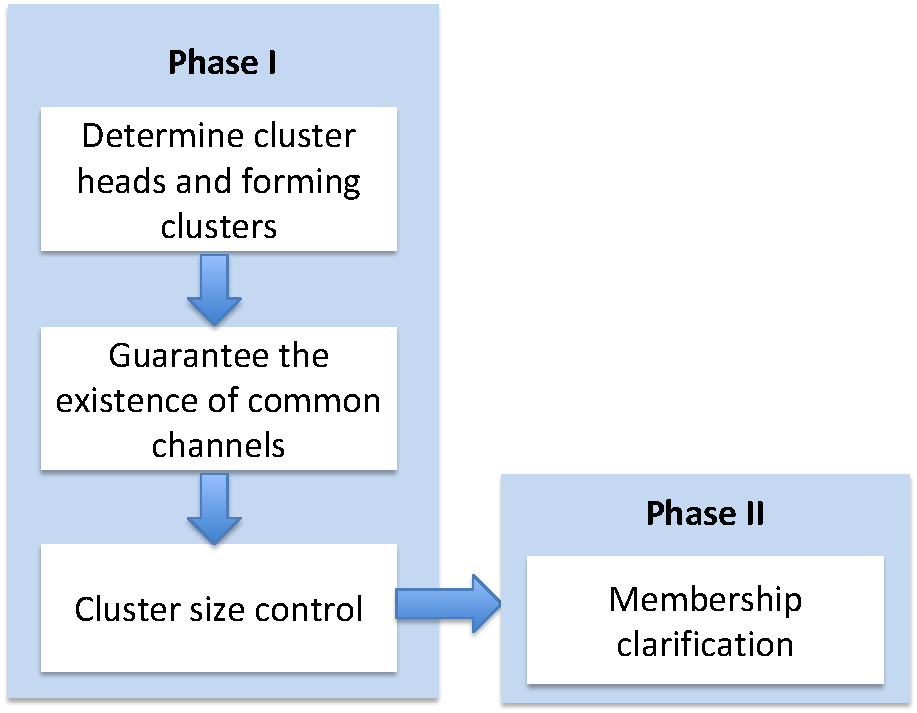
\includegraphics[width=0.9\linewidth]{flow_chart.pdf}
	\caption{Processing steps of ROSS}
	\label{flowChartROSS}
\end{figure}
In the first phase, clusters are initially formed such that every CR user becomes either cluster head or cluster member.
During this phase, size control is already realized, however, memberships might not be efficient with respect to robustness while also not being necessarily unique.
This is addressed in the second phase, where non-overlapping clusters are formed in a way that the CCs of the involved clusters are predominantly increased.

\subsection{Phase I - Cluster Formation}
\label{phaseI}
Before conducting clustering, we assume spectrum sensing and neighborhood discovery have been completed.
Furthermore, neighboring nodes have exchanged already their channel availabilities via the dedicated control channel. 
As a result, every CR node is aware of the available channels of themselves and their one-hop neighbors.
Next, cluster heads are determined after a comparison series among neighbors.
Two metrics are proposed to characterize the channel availability in the proximity of each terminal, which subsequently are used to decide the cluster heads.
\begin{itemize}

\item \textit{Individual connectivity degree} $d_i$: $d_i=\sum_{j\in \text{Nb}(i)}\vert K_i\cap K_j\vert$. 
$d_i$ is the total number of the CCs between node $i$ and each of its neighbors, it does not reflect the amount of jointly common channels among all neighbors of $i$.
\item \textit{Neighborhood connectivity degree} $g_i$: In contrast, $g_i$ is the number of CCs which are available for $i$ and all of its neighbors, thus
$g_i=|\bigcap_{j\in \text{Nb}(i)\cup i}K_j|$. It therefore represents the ability of $i$ to form a robust cluster with its neighbors.
\end{itemize}
Individual connectivity degree $d_i$ and neighborhood connectivity degree $g_i$ together form the \textit{connectivity vector} $(d_i, g_i)$.
The connectivity vector is determined by every secondary user and is then broadcasted.
Figure~\ref{fig1} illustrates the computation of the connectivity vectors for a CRN, where dashed edges indicate that the nodes are within each other's transmission range, while the number along the dashed line is the number of common channels between the two ends.
In this example, the set of available channels per terminals are given by: $K_A=\{1,2,3,4,5,6,10\}, K_B=\{1,2,3,5,7\}, \\K_C=\{1,3,4,10\}, K_D=\{1,2,3,5\}, \\K_E=\{2,3,5,7\}, K_F=\{2,4,5,6,7\}, \\K_G=\{1,2,3,4,8\}, K_H=\{1,2,5,8\}$. 
The figure shows in particular the resulting connectivity vector per node.
\begin{figure}[ht!]
  \centering
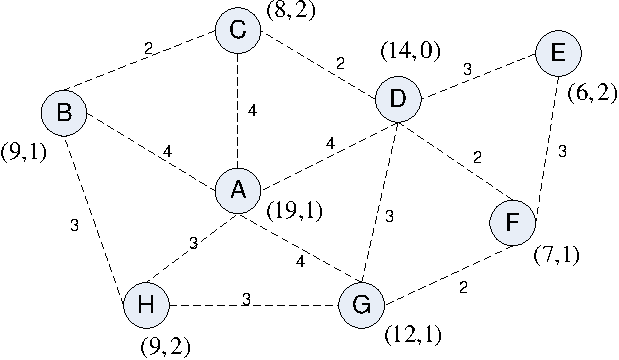
\includegraphics[width=0.7\linewidth]{figure1.pdf}
% 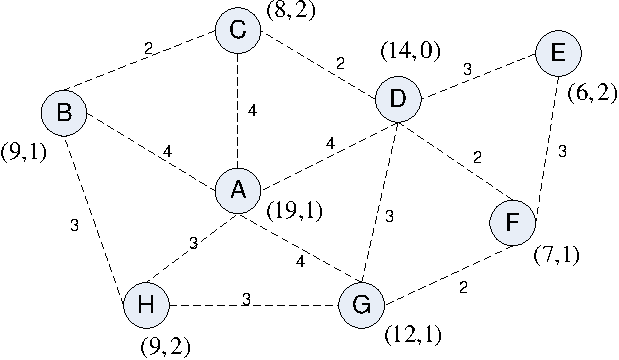
\includegraphics{figure1.pdf}
	\caption{Illustration of the resulting connectivity vector $(d_i, g_i)$ for each node of an example CRN.}
	\label{fig1}
\end{figure}

\subsubsection{Determining Cluster Heads and Forming Clusters}
Given the connectivity vector per node, the procedure of determining cluster heads is as follows.
Each CR node decides whether it is a cluster head by comparing its connectivity vector with all neighboring connectivity vectors.
When CR node $i$ has lower individual connectivity degree than any of its neighbors except for those which have already been identified as cluster heads, node $i$ becomes a cluster head.
If there is a CR node $j$ in $i$'s neighborhood, which has the same individual connectivity degree as $i$, \ie $d_j = d_i$ while the connectivity degree of $j$ is lower than for all other nodes in its neighborhood (except for nodes that already declared themselves as heads) then out of $i$ and $j$ the node with higher neighborhood connectivity degree will become cluster head.
If $g_i = g_j$ as well, the node ID is used to break the tie, \ie the one with smaller node ID becomes the cluster head.
%
The node which is identified as cluster head broadcasts a message to notify its neighbors of this status update. 
As a consequence, all neighbors - which have not become cluster head themselves -  become cluster members of this cluster head.
In this step, nodes can become member of multiple clusters, depending on how many neighbors declare themselves as cluster heads.
\footnote{The issues arising out of cluster heads in the neighborhood of a newly formed cluster head are addressed in Section~\ref{ross_p1_guarantee_ccc} and \ref{ross_p2_cluster_pruning}}
During the whole phase I, whenever a CR node becomes cluster head, or the cluster composition changes, the cluster head broadcasts new/updated information about the cluster structure, in particular the new/ update sets of available channels regarding itself and all its cluster members.
Pseudo code regarding this process, i.e. the cluster head decision and the initial cluster formation, is also provided as Algorithm~\ref{alg0} in the appendix.

After a CR node, say $i$, receives notification that there is a new cluster head in its neighborhood, $i$ sets its individual connectivity degree to a positive number $M > |\mathcal{K}| \cdot N$, and broadcasts the new individual connectivity degree. 
When node $i$ is associated with multiple clusters, \ie $i$ has received multiple notifications from different cluster heads, $d_i$ is still set to be $M$. 
The manipulation of the individual connectivity degree of the cluster members accelerates the decision on the cluster heads.





\subsubsection{The Existence of Common Channels}
\label{ross_p1_guarantee_ccc}
After executing Algorithm~\ref{alg0}, several formed clusters may not possess any CCs.
As decreasing the cluster size usually increases CCs within a cluster, the next step is to decrease the the cluster size accordingly.
This is done by following sequence of removing nodes according to an ascending list of nodes regarding their number of common channels between them and the cluster head. 
In other words, the cluster member which has the least common channels with the cluster head will be removed first.
When there are multiple nodes having the same amount of common channels with the cluster head, the node whose elimination results in more common channels will be removed.
In case of a tie, it can be broken by removing the node with smaller node ID.
It is possible that cluster heads remove all their neighbors to obtain CCs, which results in a singleton cluster.
The pseudo code for this procedure is given as Algorithm~\ref{alg_size_control_available_CCC}.
As for the nodes which are removed from a cluster, they restore their original individual connectivity degrees, then execute Algorithm~\ref{alg0} and become either cluster heads or get included into other clusters, see also Theorem~\ref{clustering:theorem}.


\subsubsection{Cluster Size Control in Dense CRN}
\label{ross_p2_cluster_pruning}

Both analysis and simulation~\cite{2017arXiv170404828L} show that with ROSS, when network density increases to a certain level, the number of formed clusters becomes constant.
This means if the network density keeps on increasing, the cluster size increases linearly with the network density.
Thus, it is necessary to control the cluster size when CRN becomes denser, and this task falls upon the cluster heads.

To control the cluster size, cluster heads remove their cluster members when cluster sizes are larger than a threshold.
The threshold should be larger than the desired size $\delta$, because there are overlaps between neighboring clusters.
%Hence, a cluster head excludes some cluster members when the cluster size exceeds a certain threshold.
We set the threshold as $t\cdot \delta$, where the constant parameter $t$ is dependent on the network density and CR nodes' transmission range.
We adopt $t$ to be between 1 and the ratio of the average neighborhood size and desired size.
When $t$ is smaller, \eg $t=1$, the formed cluster in phase I will be $\delta$.
For the cluster whose members are included by other clusters, the size of this cluster will be smaller than $\delta$ after the following membership clarification phase.
If $t$ is chosen large, \eg $t\cdot\delta$ equals the size of the neighborhood, the mechanism of adjusting the cluster size will not work any more.
	
%Because of $t$, the threshold to prune is larger than the desired size, then there will be some nodes choosing to affiliate with other clusters in the following phases.
%C1-7
The cluster head removes the cluster members sequentially according to the above explained principle.
The removed nodes restore their original individual connectivity degrees.
This process ends when each cluster's size is smaller or equal to $t \cdot\delta$.
As this procedure is similar with that in Section~\ref{ross_p1_guarantee_ccc}, Algorithm~\ref{alg_size_control_available_CCC} can also be applied.
%The $t$ is set to 1.3. 	
%C1-7

\begin{figure}[ht!]
  \centering
  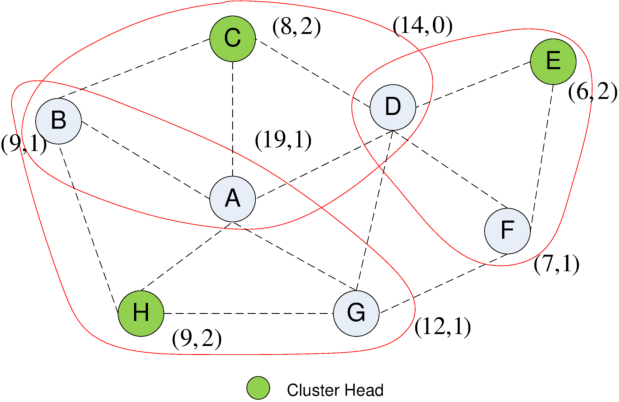
\includegraphics[width=0.5\linewidth]{figure2.pdf}
  \caption{Cluster formation after phase I of ROSS. Nodes $A, B, D$ are debatable nodes as they belong to multiple clusters.}
  \label{fig2}
\end{figure}


%%%%%%%%%%%%%%%
We have the following lemma to show every secondary user will eventually be either integrated into a cluster or become a cluster head.

\begin{lemma}
\label{clustering:lemma1}
Given a CRN where any secondary user is able to communicate with any other secondary user through the other nodes, then after the phase of cluster head selection and initial cluster formation, every secondary user either becomes cluster head, or gets included into at least one cluster.
\end{lemma}
The Proof is given in Appendix~\ref{proof_clustering:lemma1}.
%C1-6

\begin{lemma}
\label{clustering:lemma2}
When a secondary user becomes cluster head, it will not become cluster member again.
\end{lemma}
\begin{proof}
A secondary node, say $i$, becomes cluster head when its \textit{individual connectivity degree} is smaller than any of its neighbors.
Afterwards, the \textit{individual connectivity degrees} of its neighbors becomes $M$.
%If all the neighbors stay in the cluster, the cluster head will remain to be cluster head.
If certain nodes are removed from the cluster due to guaranteeing CC or size control, these nodes may become either cluster members of another cluster head, or cluster heads themselves.
In both cases, $i$'s \textit{individual connectivity degree} is still smaller than the one of the respective other nodes.
Note that when the removed node becomes cluster head, it will not include its former cluster head $i$, so that $i$ doesn't become cluster member and so its \textit{individual connectivity degree} doesn't change.
\end{proof}


\begin{lemma}
\label{clustering:lemma3}
In the process of cluster head selection and initial cluster formation, the maximum number of times that a secondary node becomes cluster head is $N$.
\end{lemma}
This lemma follows from Lemma~\ref{clustering:lemma2} considering that $N$ is the number of all the secondary users in the CRN.
Based on the above lemmas, we have:
\begin{theorem}
\label{clustering:theorem}
Assuming the time for a secondary user to update the information about cluster heads in its neighborhood is $T$, then it takes at most $N*T $ to finish the process of cluster head selection and initial cluster formation.
\end{theorem}
Phase I ends when no more secondary users become cluster heads.
Based on Lemma~\ref{clustering:lemma1} and Lemma~\ref{clustering:lemma3}, Theorem~\ref{clustering:theorem} follows directly.
Note that as Algorithm~\ref{alg0} is executed concurrently by different secondary users, the required time is typically considerably lower.

If we apply Algorithm~\ref{alg0} to the example CRN in Figure~\ref{fig1}, the outcome results to the representation in Figure~\ref{fig2}.
Node $B$ and $H$ have the same individual connectivity degree, i.e., $d_B=d_H$. As $g_H=2>g_B=1$, node $H$ becomes the cluster head and cluster $C(H)$ is $\{H, B, A, G\}$.


\subsection{Phase II - Membership Clarification}
\label{membershipClarification}
%\subsubsection*{Problem Description}
After running phase I of ROSS, we notice that nodes $A, B, D$ are included in more than one cluster as shown in Figure~\ref{fig2}. 
We refer to these nodes as \textit{debatable nodes} as their cluster affiliations are not uniquely decided.
All clusters which include debatable node $i$ are called \textit{claiming clusters} of node $i$, and the set of these clusters is denoted as $S_i$.  
Nevertheless, debatable nodes need to be exclusively associated with only one cluster and be removed from the other claiming clusters.
We refer to this procedure as \textit{cluster membership clarification}.

\subsubsection{Distributed Greedy Algorithm (DGA)}
When a debatable node $i$ decides to join cluster $C\in S_i$, the guiding idea is that its decision should result in the greatest increase of CCs in all its claiming clusters.
As node $i$ has been notified of the spectrum availability on all the nodes in each claiming cluster, node $i$ is able to calculate how many more CCs will result in a claiming cluster if $i$ leaves that cluster.
Then node $i$ decides on the cluster $C\in S_i$, if $i$ leaving cluster $C$ results in a lower increase in terms of CCs than leaving any other claiming clusters in $S_i$.
%As to a cluster $C\in S_i$, if $i$ leaves cluster $C$ and results in less increased CCs than leaving any other claiming clusters, then $i$ chooses to stay in cluster $C$.
In case of a tie between two claiming clusters, $i$ chooses to stay in the cluster whose cluster head shares the most CCs with $i$.
When a tie still exists, node $i$ chooses to stay in the claiming cluster which has the smallest size.
Node IDs of cluster heads will be used to break tie in the end if necessary.
The pseudo code of this algorithm is given by Algorithm~\ref{alg4}.
After deciding its membership, debatable node $i$ notifies all its claiming clusters.
%xxxxxxxxxxxxxxxxxxx

The autonomous decisions made by the debatable CR nodes raises the possibility of an endless chain effect during the membership clarification phase.
A debatable node's choice is dependent on the composition of its claiming clusters, and the members of these claiming clusters can be changed by other debatable nodes' moves.
There is the possibility that this process may go on forever.
However, by formulating the process of membership clarification into a game, we can show that an equilibrium is reached after a finite number of best response updates made by the debatable nodes.
Thus, the membership clarification phase is guaranteed to terminate.


\subsubsection{Bridging ROSS-DGA with Congestion Game}
\label{clustering:phaseII:game}
Game theory is a powerful mathematical tool for studying, modeling and analyzing the interactions among individuals.
A game consists of three elements: a set of players, a selfish utility for each player, and a feasible strategy space for each player. 
In a game, the players are modeled as rational and intelligent decision makers, which are related through one explicit formalized incentive expression (the utility or cost).
Game theory provides standard procedures to study potential equilibria~\cite{game_for_communication_01}.
Over the last decade, game theory has been extensively applied to problems in communication and networking~\cite{Neel06analysisand, Wang_gtc_crn_survey_2010}.
Congestion game is an interesting game model which describes the problem where participants compete for limited resources in a non-cooperative manner.
It has the good property that a Nash equilibrium can be achieved after finite steps of best response dynamic, \ie each player chooses the strategy to maximize/minimize its utility/cost with respect to the other players' strategies.
The framework of the congestion game has been used to model server selection in distributed computing platforms~\cite{Cloud_Computing_2010}, or users downloading files from cloud, etc.

To formulate the debatable nodes' membership clarification into a congestion game, we reexamine this process from a different perspective. 
Thus, debatable nodes are not included in any cluster and they need to decide on one cluster to join.
When a debatable node $i$ joins one cluster $C$, the decrease of CCs in cluster $C$ is $\sum_{C\in S_i}\Delta\vert K(C) \vert=\sum_{C\in S_i}({\vert K(C) \vert-\vert K(C\cup i) \vert})$.
Then, node $i$ chooses the cluster $C$, where the decrease of CCs in cluster $C$ is smaller than the decrease if $i$ would have joined any other claiming cluster in $S_i$.
The relation between the debatable nodes and the claiming clusters is shown in Figure~\ref{debatable_nodes_claiming_cluster}.

\begin{figure}[ht!]
  \centering
  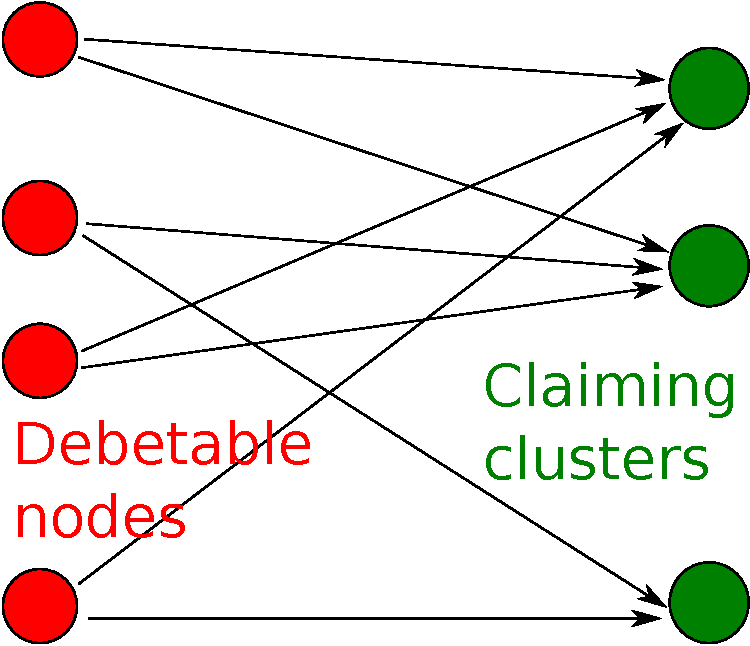
\includegraphics[width=0.37\linewidth]{singletongame_matching.pdf}
  \caption{Illustration of debatable nodes and claiming clusters}
  \label{debatable_nodes_claiming_cluster}
\end{figure}


In the following, we show that the decision of debatable nodes to clarify their membership can be mapped to the behaviour of the players in a \textit{player-specific singleton congestion game} when proper cost function is given.
The game to be constructed is represented with a 4-tuple $\Gamma=(\mathcal{P},\mathcal{R},\sum_{i, i \in \mathcal{P}}, f)$ with the following elements:

\begin{itemize}
	\item $\mathcal{P}$, the set of players in the game, which are the debatable nodes in our problem.
	\item $\mathcal{R} = \cup S_i, i\in \mathcal{P}$, the set of the resources for players to choose. In our problem, $S_i$ is the set of the claiming clusters of $i$, and $\mathcal{R}$ is the set of all claiming clusters.
	\item Strategy space $\sum_i, i \in \mathcal{P}$, $\sum_i$ is the set of the claiming clusters $S_i$.
	As debatable node $i$ is supposed to choose only one claiming cluster, only a single resource will be allocated to $i$.%, accordingly this congestion game is a singleton game.
	\item 	The cost function $f(C)$ regarding resource $C$. 
	$f(C) = \Delta\vert K^i(C)|, C\in S_i$, which represents the decreased number of CCs in cluster $C$ when debatable node $i$ joins $C$.
	As to cluster $C\in S_i$, the decrease of CCs caused by accepting the debatable nodes is $\sum_{i:C\in S_i, i\rightarrow C} \Delta\vert K^i(C) \vert$. 
$i\rightarrow C$ means $i$ joins cluster $C$.
Obviously this function is non-decreasing with respect to the number of nodes joining cluster $C$.
	
When the utility function is decided purely by the amount of players accessing the resource, the game is a canonical congestion game~\cite{Ackermann06purenash}.
In our game, as the channel availability on debatable nodes (players) is different, the loss of CCs (cost) caused by a debatable node could also be different.
%For example, given two same groups of debatable nodes and their sizes are the same, when the nodes are not completely the same (neither are the channel availabilities on these nodes), the cost happened on one claiming cluster could be different if the two groups of debatable nodes join that cluster respectively.
Hence, this congestion game is player specific~\cite{Ackermann06purenash}.
In this game, every player greedily updates its strategy (choosing one claiming cluster to join) if joining a different claiming cluster minimizes the decrease of CCs $\sum_{i:C\in S_i} \Delta\vert K^i(C) \vert$, and a player's strategy in the game is exactly the same with the behaviour of a debatable node in the membership clarification phase.


%	\item The Rosenthal's potential function \cite{Rosenthal} of this congestion game is given by:
%	\begin{equation*}
%	\phi(S)=\sum_{C\in\mathcal{R}} \sum_{i:C\in S_i} \Delta\vert K^i_C \vert   	
%   	%\sum_{i=1}^N \Delta^{i}_{p}(S)=\sum_{i=1}^N \sum_{r\in S_i}\Delta^{i}_{r}(t)	
%  	% \Delta =\sum_{i=1}^N w_i (x_i - \bar{x})^2 .
%	\end{equation*}
%All the players in this game greedily update their strategy to minimize the potential function (congestion), this process is exactly the same with the network behaviour under \textit{Distributed Greedy Algorithm}. 

%	\item It is an asymmetric game because the sets of strategies shared by different players are different.
%	\item The total cost is: 
%\begin{equation*}
%   \sum_{i=1}^N \Delta^{i}_{p}(S)=\sum_{i=1}^N \sum_{p\in s_i} \Delta^{i}_{p}(n_p(S))
%  % \Delta =\sum_{i=1}^N w_i (x_i - \bar{x})^2 .
%\end{equation*}

%This is the global objective we want to minimize.
\end{itemize}

%Singleton congestion game is a special type of matroid game~\cite{Milchtaich1996111,}. 
%It is known that player-specific matroid congestion game admit pure equilibrium, 

As to singleton congestion game, there exists a pure equilibrium which can be reached with the best response update, while the upper bound for the number of steps before convergence is $n^2*m$~\cite{Ackermann06purenash}, where $n$ is the number of players, and $m$ is the number of resources.
In our problem, the players are the debatable nodes, and the resources are the claiming clusters.
Thus, the number of steps can be expressed as $\mathcal{O}(N^3)$.
%
In fact, the upper bound for the number of steps which are involved in this process is much smaller than $N^3$.
The percentage of debatable nodes in the network is shown in Figure~\ref{percentage_overlapping_node}, which is between 10\% to 60\%.
On the other hand, the number of cluster heads is dependent on the network density and the CR node's transmission range, as mentioned in Section~\ref{phaseI}.
The simulation in \cite{robust_clustering_arxiv} shows that the cluster heads account for from 3.4\% to 20\% of the total CR nodes with increasing network density.
Furthermore, as the game is played locally and in parallel \ie a debatable node can only interact with a few claiming clusters, the execution speed is significantly reduced.


\subsubsection{Distributed Fast Algorithm (DFA)}
On the basis of ROSS-DGA, we propose a faster version ROSS-DFA which differs from ROSS-DGA in the second phase.
With ROSS-DFA, debatable nodes decide their respective cluster heads only once.
The debatable nodes consider their claiming clusters to include all their debatable nodes, thus the membership of claiming clusters is static and all the debatable nodes can make decisions simultaneously without considering the change of membership of their claiming clusters.
As ROSS-DFA is quicker than ROSS-DGA, it is more suitable for CRN where the channel availability changes frequently.
To run ROSS-DFA, debatable nodes execute only one loop of Algorithm~\ref{alg4}.

Now we apply both ROSS-DGA and ROSS-DFA to the network in Figure~\ref{fig2} after phase I of ROSS is complete.
%C1-8
In the network, node $A$'s claiming clusters are cluster $C(C), C(H)\in S_A$, while the respective members are $\{A,B,C,D\}$ and $\{A,B,H,G\}$. 
The two possible strategies of node $A$ are illustrated in Figure \ref{fig3}.
In Figure \ref{AinC}, node $A$ stays in $C(C)$ and leaves $C(H)$ which brings 2 more CCs to $S_A$, which is more than that brought by another strategy, as shown in \ref{AinH}.
After similar decisions are made by the other debatable nodes $B$ and $D$, the final clusters are formed as shown in Figure~\ref{final_clustering_ross}.

%Using DFA in phase II, the time complexity is decreased drastically to 1. Thus, the total complexity of ROSS-DFA is $|I|$, while, ROSS-DGA's complexity is $|I|^3$ in the worst case.


\begin{figure}[h]
\centering
\subfigure[Node A stays in cluster $C(C)$, quits $C(H)$, $\Delta\vert K(C(C))\vert+\Delta\vert K(C(H))\vert=2$]{
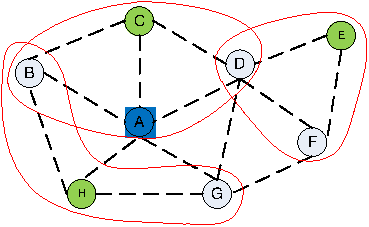
\includegraphics[width=0.435\linewidth]{figure4AinC.pdf}
\label{AinC}
}
\hspace{.15 in}
\subfigure[Node A stays in cluster $C(H)$, quits $C(C)$, $\Delta\vert K(C(C))\vert+\Delta\vert K(C(H))\vert=1$]{
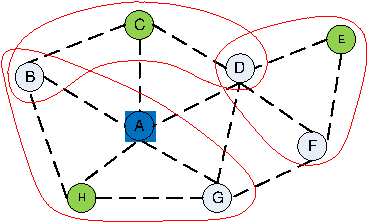
\includegraphics[width=0.435\linewidth]{figure4AinH.pdf}
\label{AinH}
}
\caption[]{Membership clarification: possible cluster formations caused by node A's different choices} %\subref{node A in $C_C$}, \subref{node A in $C_H$}}
\label{fig3}
\end{figure}


\begin{figure}[h]
  \centering
  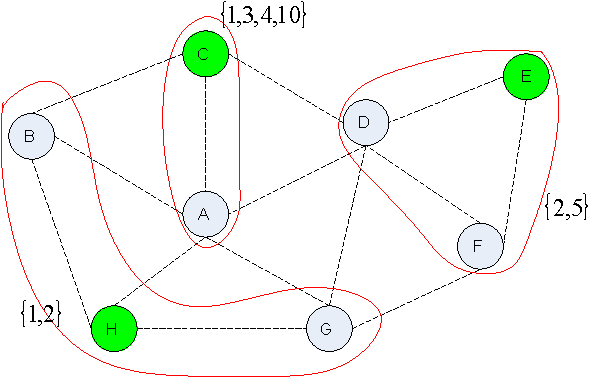
\includegraphics[width=0.5\linewidth]{final_clustering_ross.pdf}
  \caption{Final formation of clusters. Common channels are shown as well as the corresponding clusters.}
  \label{final_clustering_ross}
\end{figure}




\section{Performance Evaluation}
\label{performance}
Taking the final clustering result of ROSS into account for our toy example shown in Figure~\ref{final_clustering_ross}, we can compare the outcome with our centralized scheme proposed in Equation~\ref{centralized_opt} as well as the state-of-the-art algorithm SOC~\cite{LIU_TMC11_2}.
Those corresponding results of the later two schemes are shown in Figure~\ref{fig:final_clustering}.
We observe for this example case that ROSS and the centralized scheme achieve cluster sizes that are more balanced, while SOC leads to a larger variance in terms of the cluster size.
Regarding the amount of CCs, the same observation holds. 
\begin{figure}[ht]
\begin{center}
\subfigure[Generated by SOC]{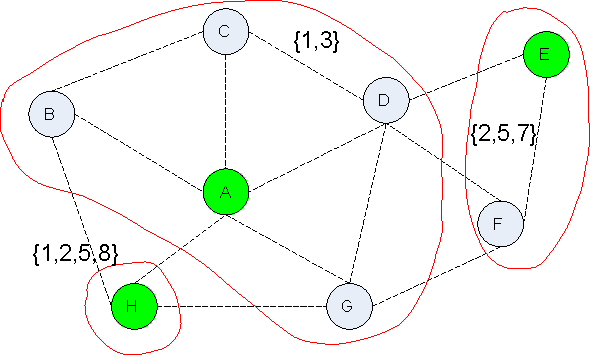
\includegraphics[width=0.435\linewidth]{final_clustering_soc}\label{fig:final_clustering_soc}}
\hspace{0.15 in}
\subfigure[Generated by the centralized clustering scheme]{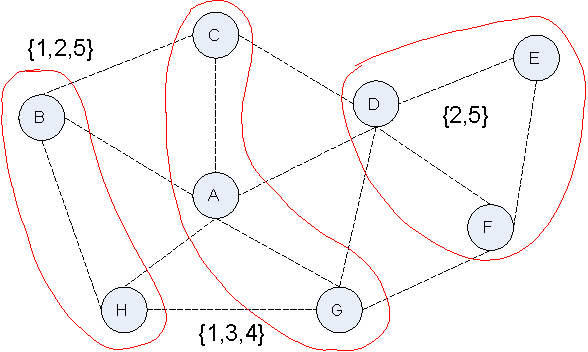
\includegraphics[width=0.435\linewidth]{final_clustering_LP}\label{fig:final_clustering_LP}}
\end{center}
\caption{Final clusters formed by SOC as well as the centralized clustering scheme.}
\label{fig:final_clustering}
\end{figure}

In the following, we are interested in a more general performance comparison regarding clustering in CRNs.
We therefore present in the following an extensive evaluation study.
We base our evaluations on simulations, and consider the following comparison schemes:
\begin{itemize}
\item ROSS without size control: ROSS-DGA, ROSS-DFA;
\item ROSS with size control, \ie ROSS-$\delta$-DGA and ROSS-$\delta$-DFA where $\delta$ is the desired cluster size;
\item SOC~\cite{LIU_TMC11_2}, a distributed clustering scheme pursuing cluster robustness;
\item Centralized robust clustering scheme; in our evaluations we use the built-in function $bintprog$ of MATLAB to solve the corresponding integer optimization problem given in Equation~\ref{centralized_opt}
\end{itemize}

Given these comparison schemes, we are interested in the following performance metrics regarding clustering:
\begin{itemize}
\item \textbf{The average number of CCs per non-singleton cluster.}
Previous work \cite{LIU_TMC11_2} and \cite{Li11_ROSS} claim that the larger average number of CCs over all the clusters indicates robustness. As mentioned, this interpretation has several shortcomings:
First, singleton clusters should not be considered when calculating the average number of CCs, as singleton clusters don't contribute to the collaborative computing or sensing.
Second, the average number of CCs doesn't necessarily indicate the robustness of a cluster, because the ability of a cluster to sustain primary user activity also depends on the size and the location of the cluster members. This information, however, is not reflected by the average number of CCs.
Thus, in the following we will consider the average number of CCs per cluster, excluding singleton clusters from this averaging, as our first performance metric.
\item \textbf{Robustness of the clusters against newly added PUs.}
If clusters are less robust, this leads to an increasing number of unclustered CR nodes if clusters are exposed to random primary user activity.
We thus are interested in this effect as a second measure for robustness. 
In particular, we are interested in the number of CR nodes which are still part of a cluster after exposing the clusters to primary user activity.
\item \textbf{Cluster sizes.}
We investigate the distribution of the size the formed clusters.
This metric reflects that above mentioned size constraints, i.e. clusters are supposed to be neither too big nor too small.
\item \textbf{Control message overhead.}
We investigate the number of control messages involved until the final clustering result is established .
\item \textbf{Influence from inaccurate spectrum sensing.}
While most of our evaluations are conducted under the assumption of perfect channel sensing by the individual CR nodes, an important question relates to the fact how the clustering performs under imperfect sensing accuracy.
In case of erroneous channel sensing, false negatives harm primary users while false positives harm the CR nodes.
Both effects obviously impact the clustering process. 
However, in the following we only consider the impact from false negatives. 
In particular, we assume that primary user activity is only correcly detected by a CR node in transmission range with a certain probability, i.e. there is a certain probability for misdetections.
Given this erroneous sensing result, the secondary users nevertheless make their clustering decisions.
As we are interested in the distorting impact of the erroneous channel sensing results on the clustering process, after the clustering is complete, we provide ground truth and reevaluate the discrepancy between the assumed channel utilization and its effect on clustering, and the de-facto channel utilization and how this affects the CCs of formed clusters.
\end{itemize}

Our performance evaluation is split into two parts:
First we investigate the performance of the centralized scheme and the distributed schemes for a small network, as the run-time for the centralized solution quickly grows out of hand as a function of the network size .
In the second part, we investigate the performance only of the distributed schemes for larger settings.
The following simulation settings are identical for both evalutions:
CRs and PUs are deployed on a two-dimensional Euclidean plane.
%Complying with the system model, the CR node residing within another CR node's transmission range is seen as neighbour of that CR node.
The number of licensed channels is 10, each PU is operating on each channel with probability of 50\%.
%C1-10
The constant $t$ which is used to control cluster size for ROSS (discussed in Section~\ref{ross_p2_cluster_pruning}) is 1.3.
CR users are assumed to sense the existence of primary users and identify available channels perfectly, unless we investigate the impact from erroneous channel sensing.
All primary and CR users are assumed to be static during the process of clustering.
All other parameters \ie the number of CR and PU, and their transmission ranges are given at the beginning of the respective subsections.
The simulation is written in C++, and the performance results are averaged over 50 randomly generated topologies.
We provide confidence interval corresponding to a 95\% confidence level.

\subsection{Centralized Schemes vs. Decentralized Schemes}
We start with the comparison of the centralized scheme versus various distributed ones.
For this, we consider 10 primary users and 20 CR users are dropped randomly (with uniform distribution) in a square area where side length is $A$.
Transmission ranges of both primary and CR users are set to $A/3$.
By doing this, we abstract from the influence of any given physical layer technology and propagation environment parameters.
Due to the parameterization, on average 7 channels are available per CR node when the clustering process is started.
We set the desired cluster size $\delta$ as 3.
As for the centralized scheme, we set the following parameters numerically: $\rho_1 =  0.4$, $\rho_2 =  0.6$.

We start with the consideration of the CCs in all non-singleton clusters.
Figure~\ref{ccc_per_nonsingleton} shows that basically the centralized schemes outperforms all distributed schemes in terms of the average number of CCs per cluster.
SOC achieves the most CCs among the distributed schemes, because SOC groups the neighboring CRs which share the most abundant spectrum together, without considering the size of them.
%We have discussed the flaw of this metric as it doesn't convey the number of unclustered CR nodes, in fact, 
However, as a consequence, SOC also generates the most singleton clusters.
As to the variants of ROSS, we notice that the greedy mechanism (i.e. the ROSS-DGA variants) maximize the CCs in non-singleton clusters significantly.
\begin{figure*}[th]
\begin{multicols}{3}
    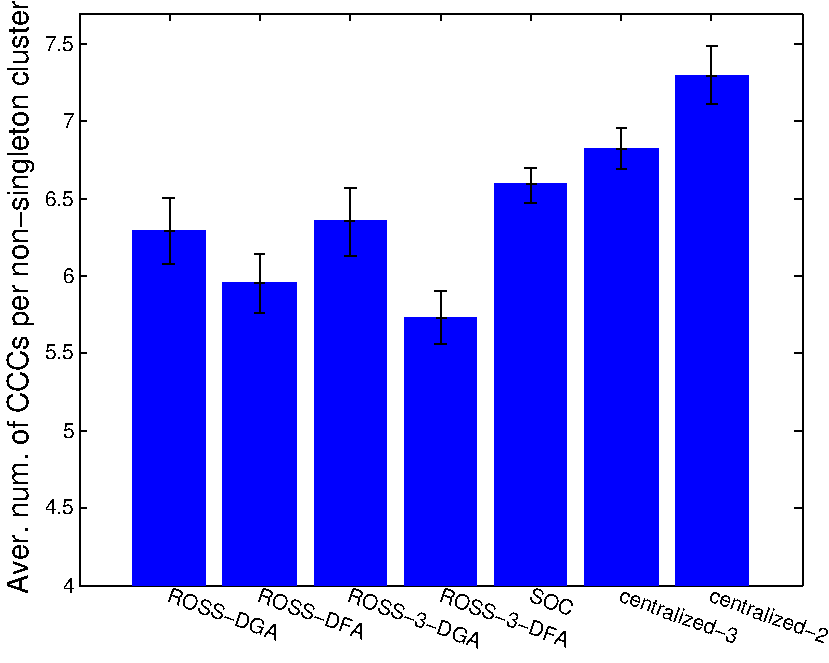
\includegraphics[width=\linewidth]{ccc_20.pdf}\par\caption{Average number of CCs of non-singleton clusters}\label{ccc_per_nonsingleton}
    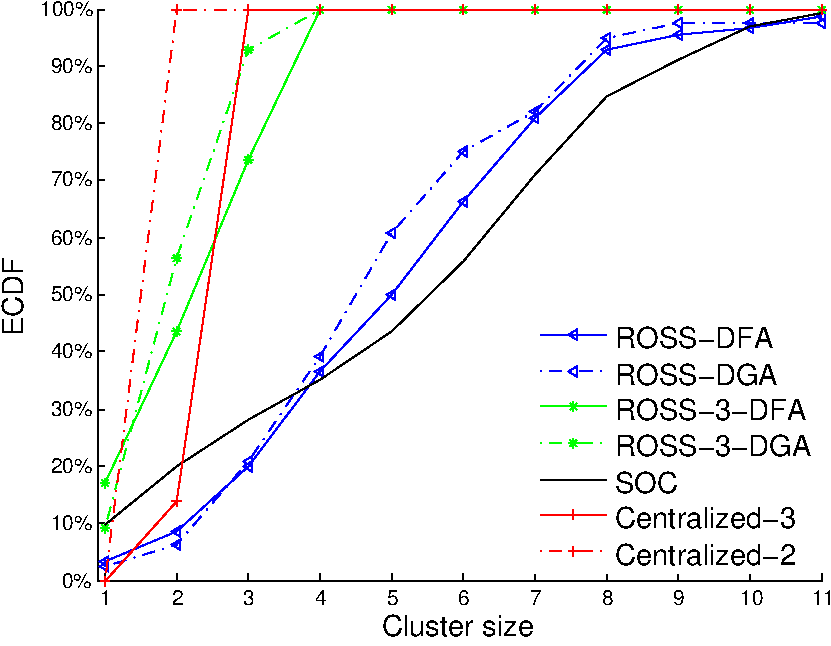
\includegraphics[width=\linewidth]{cdf_clusterSize_20.pdf}\par\caption{Cumulative distribution of CRs residing in clusters with different sizes}\label{size_control}    
    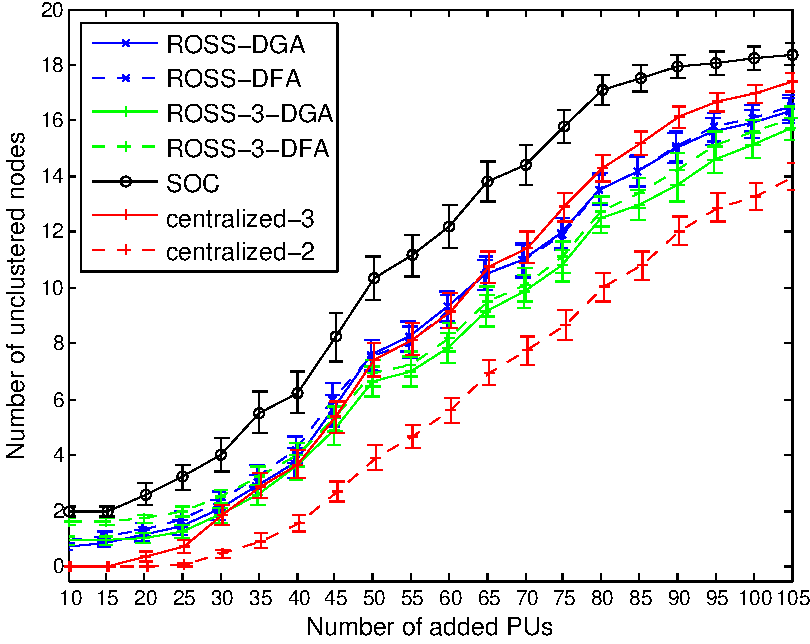
\includegraphics[width=\linewidth]{survival_rate_20.pdf}\par\caption{Number of unclustered CRs with decreasing spectrum availability}\label{singleton_clusters}
\end{multicols}
\label{compare_dis_centralized}
\end{figure*}

Figure~\ref{size_control} provides further insights into the performance comparison.
Here, we depict the empirical cumulative distribution function of the size of the clusters.
%First, given the channel availability in the CRN, SOC generates more unclustered CR nodes than other schemes.
The centralized schemes don't result in any singleton clusters in the the considered evaluation scenarios.
In contrast, ROSS-DGA/DFA account for 3\% singleton clusters of the total CR nodes, as compared to 10\% of nodes being unclustered when applying SOC.
ROSS-DGA and ROSS-DFA with size control feature generate 5\%-8\% unclustered CR nodes, which is due to the cluster pruning procedure (discussed in Section~\ref{ross_p1_guarantee_ccc} and Section~\ref{ross_p2_cluster_pruning}).
In terms of cluster size, the clusters resulting from the centralized schemes and ROSS with cluster size control mechanism have little deviation from the desired cluster size.
In contrast, the size of clusters resulting from ROSS-DGA and ROSS-DFA have a higher variance, but appear to be better than SOC, i.e., the 50\% percentiles for ROSS-DGA, ROSS-DFA and SOC are 4.5, 5, and 5.5, and the 90\% percentiles for the three schemes are 8, 8, and 9.
Thus, the corresponding sizes resulting from ROSS are closer to the desired size.

Next, we consider the robustness of clusters if facing random primary user activity.
We thus extend the simulation by adding more primary users sequentially into CRN, leading to a decreasing spectrum availability.
While 10 primary users are in the network at start, some extra19 batches of primary users are added sequentially, each batch including 5 primary users that are placed randomly in the area.
These added primary users choose then an active channel also at random. 
Figure~\ref{singleton_clusters} shows the corresponding average number of unclustered CR nodes as a result of this significant increase in primary user activity. 
The figure reveals that the centralized scheme with a desired size of 2 leads to the best robustness, while SOC leads to the worst one.
Surprisingly, the centralized scheme with desired size of 3 doesn't outperform the variants of ROSS, because pursuing larger cluster sizes generally leads to clusters with a lower amount of CCs. 
In contrary, the variants of ROSS generate some smaller clusters which are more likely to be maintain despite the increasing primary user activity.

Alternatively, we can consider the total share of users (still) residing in a cluster after the addition of the primary users as performance metric for robustness.
If we do so, the ROSS-based schemes maintain 5\%, 30\% and 230\% more secondary users within clusters than SOC, when the numbers of newly added PR are 10, 40 and 80 respectively (no figure is provided for this data).
%XXXXX
The above observation illustrates clearly that the average number of CCs of non-singleton clusters doesn't necessarily reflect the robustness of clusters, \ie SOC obtains the most CCs among the distributed schemes, but the resulting clusters are vulnerable to primary user activity.

We finally turn to a comparison of the involved signaling overhead for the different clustering schemes.
For this, we count the number of \textit{transmissions of control messages} as metric~\cite{complexity_aggregation_2011}, without distinguishing broadcast or uni-cast control messages.
%In Section~\ref{ross}, this metric is synonymous with the \textit{the number of updates}.
%We don't consider the the control messages which are involved in neighborhood discovery, which is the premise and deemed to be the same for all clustering schemes.
%According to~\cite{complexity_aggregation_2011}, the message complexity is defined as the number of messages used by all nodes.

As to ROSS, in the first phase the maximal number of broadcast is $N$ according to~\ref{clustering:theorem}.
The upper limits for the message exchanges are $n^2m$ and $n$ for ROSS-DGA and ROSS-DFA, respectively.
SOC consists of three rounds, and in each round every node needs to perform a broadcast to do comparisons and cluster merging.
The centralized scheme is conducted at some control device, which involves information aggregation and subsequent dissemination of clustering decisions.
To analyze the centralized scheme's message overhead, we adopt a backbone structure proposed in~\cite{Efficient_broadcasting_gathering_adhoc}, and apply ROSS to generate cluster heads which serve as the backbone.
In the stage of information aggregation, all the nodes transmit information to the cluster heads which forward the messages to the controller. 
In the dissemination stage, all the cluster heads and the debatable nodes broadcast the clustering result, thus the upper limit for the number of broadcast is $N+m+n$.

The number of control messages which are involved in ROSS variants and the centralized scheme is related to the number of debatable nodes.
Figure~\ref{percentage_overlapping_node} shows the percentage of debatable nodes with different network densities.
\begin{figure}[ht!]
  \centering
  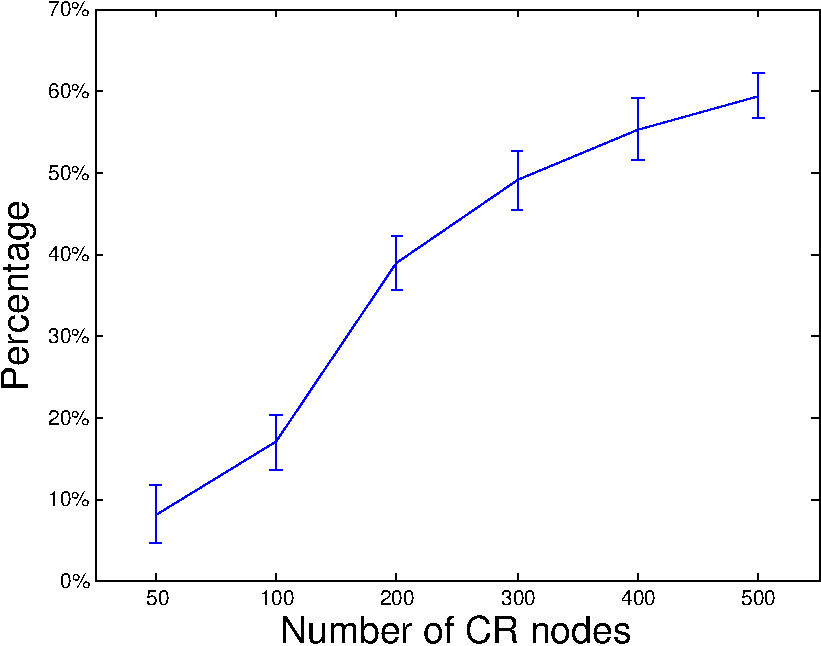
\includegraphics[width=0.6\linewidth]{percentage_overlapping_node.pdf}
  \caption{Percentage of debatable nodes after phase I of ROSS.}
  \label{percentage_overlapping_node}
\end{figure}
%
%As we adopt a simplified communication model, node's transmission is not influenced by collision or interference, 
%Our simulation doesn't consider the behaviour in the physical layer, 
%
%
%Assume we use OSPF~\cite{BCJ10} to aggregate and disseminate information, then the best and worst complexity for is $\mathcal{O}(E)$, where $E$ is the number of edges in the graph which corresponds to the network.
%The minimum number of edges is $n-1$ when the nodes form a line and each node has at more two neighbours, and the maximum number is $N*(N-1)/2$ when the nodes form a complete graph.
%Thus the best message complexity of the centralized scheme is $\mathcal{O}{(N)}$ and the worst is $\mathcal{O}{(N^2)}$.
%
%1. update membership to form X1, 
%2. broadcast new X1, form new X2
%3. broadcast X3
%The complexity parameters are the number of nodes $n$ in network, number of clusters $h$.
Table \ref{tab_overhead} shows the messaging overhead , quantitative amount of control messages, and size of control messages for the different schemes under consideration.
Figure~\ref{control_msg} shows the analytical result of the amount of transmissions involved in different schemes.
%the upper bound of the number of transmissions of ROSS, and the analytic number of transmissions of the centralized scheme. 

\begin{center}
\begin{table*}[!htb]
\caption{Signalling overhead}\label{tab_overhead}
{\renewcommand{\arraystretch}{1.15} %<- modify value to suit your needs
{\small
\hfill{}
\begin{threeparttable}
\begin{tabular}{|C{1.8 cm}|C{2.6 cm}|C{3 cm}|C{6.3 cm}|}
\hline
 Scheme 				&Message Overhead 	&   Quantitative number of messages 		& Content and size of the message 									\\ \hline
 ROSS-DGA, ROSS-$\delta$-DGA 	&$\mathcal{O}(N^3)$ (worst case)		&   $N+n^2m$ (upper bound)  				&   \multirow{2}{*}{\parbox{7.7cm}{PhaseI: ID, $d_i$,$g_i$, which are 3 bytes;\\ PhaseII: Cluster head $i$ broadcasts channel availability to all \\ members, where are $|C(i)| |\mathcal{K}|$ bytes}}								\\ \cline{1-3}
 ROSS-DFA, ROSS-$\delta$-DFA 	&$\mathcal{O}(N)$ (worst case)		&   $N + n$	 (upper bound) 					& 	      												\\ \hline
 SOC 					&$\mathcal{O}(N)$		&   $3N$									& Every CR node $i$ broadcasts channel availability on all cluster members, which is $|C(i)| |\mathcal{K}|$ bytes
 \\ \hline
 Centralized			&$\mathcal{O}(N)$			&	$N + n + m$ (upper bound) 		& clustering result, which is 2$N$ bytes \tnotex{tnote:robots-r1} 					\\ \hline
\end{tabular}
    \begin{tablenotes}
      \item\label{tnote:robots-r1}Assuming the data structure of the clustering result is in the form of $\{i, C\}, i\in C, i\in \mathcal{N}$.
    \end{tablenotes}
    \end{threeparttable}
}
}
\hfill{}
\end{table*}
\end{center}

\begin{figure}[ht!]
  \centering
  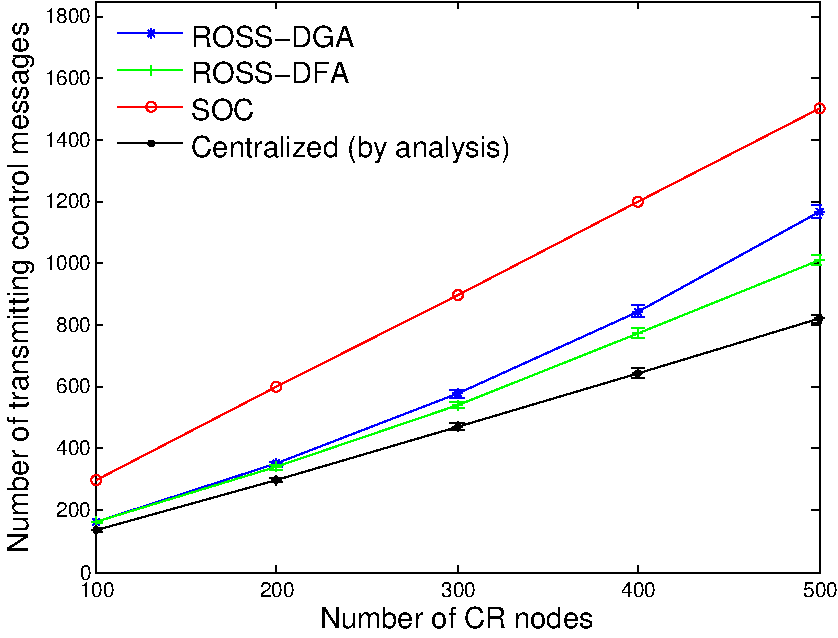
\includegraphics[width=0.6\linewidth]{number_controlMsg.pdf}
  \caption{Absolute amount of control messages required for clustering.}
%XXXXXX Quantitative, or Absolute
  \label{control_msg}
\end{figure}





\subsection{Comparison among the Distributed Schemes}
\label{largeScaleCRN}
We now switch to a more fine-grained investigation only of the distributed schemes. 
We are here most important interested in their properties when the network size and density scales.
In our scenario, we set now the transmission range of CR to $A/5$ while the primary user transmission range is set to $2A/5$.
The initial number of primary users is set to 30.
%The number of CR is 100, 200 and 300, and the average number of neighbours of each CR is 9.5, 20, and 31.
As we scale now the number CR nodes in the scenario, we adjust the desired size in the clustering process.
Our adopted values are listed in the Table~\ref{Simulation_para}, which represent about 60\% of the average number of neighbors.
%When run ROSS, the parameter $t$ which is used to control cluster size in phase I is 1.3.

\begin{table}[ht]
\caption{}
\label{Simulation_para}
{\small
%\hfill{}
\begin{tabular}{|L{3 cm}|C{0.85 cm}|C{0.85 cm}|C{0.85 cm}|}
\hline
Number of CRs			& 100 	&  200 					& 300 \\ \hline
Average num. of neighbors 	&9.5	&   20		& 31  \\ \hline
Desired size $\delta$ 	& 6	&   12 						& 20      \\ \hline
\end{tabular}
}
%\hfill{}
\end{table}



\subsubsection{Number of CCs per Non-singleton Clusters}

\begin{figure}[ht!]
  \centering
  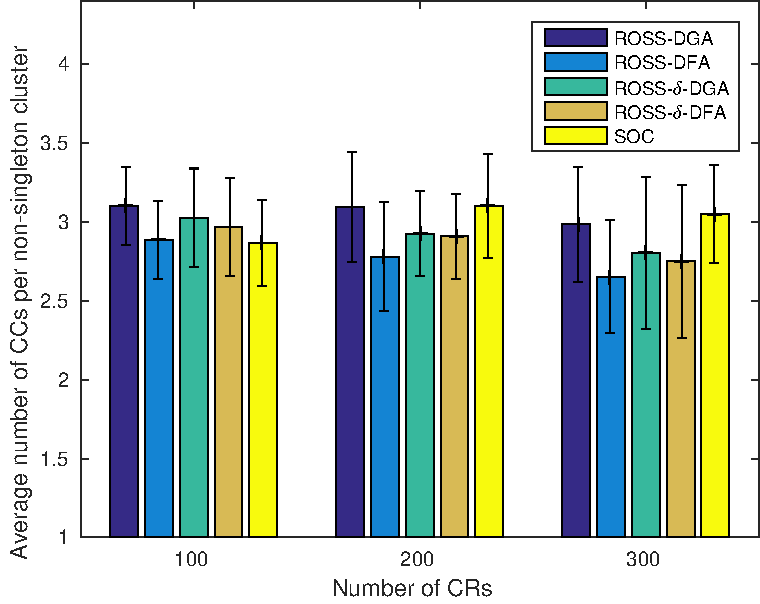
\includegraphics[width=.7\linewidth]{ccc_large_scale_color_082017_newdata_no_texture.pdf}
  \caption{Average number of CCs of non-singleton clusters in case of increasing the number of CR nodes.}
  \label{ccc_large_scale}
\end{figure}
We start again with considering the average number of CCS over all non-singleton clusters, shown in Figure~\ref{ccc_large_scale}.
Note that in this case we increase the number of CR nodes in the scenario.
The result does not reveal, as in the previous section, a significant performance advantage of either of the distributed schemes.

We next consider the robustness of the formed clusters in case that more and more primary users are added to the scenario.
In this case, we increase primary users' activity by adding 20 batches of primary users sequentially in CRN, each batch including 10 primary users which are placed randomly and select a channel at random. 
Figure~\ref{singleton_clusters_100} and \ref{singleton_clusters_200} show the corresponding results for $N=100$ and 200 CR nodes in the scenario.
We basically see that as the primary user activity increases, more unclustered CR nodes result from SOC than the variants of ROSS.
This correlates a somewhat similar observation in the previous section.
When $N=300$, as shown in Figure~\ref{singleton_clusters_300}, and the amount of newly added primary users is moderate, ROSS-DGA/DFA results in slightly more unclustered CR nodes than SOC, while SOC's performance deteriorates quickly when the number of primary users continue increasing.
Also, Figures~\ref{singleton_clusters_100} to~\ref{singleton_clusters_300} reveal that ROSS with size control mechanism results in significantly less singleton clusters.
\begin{figure*}[t]
\begin{multicols}{3}
    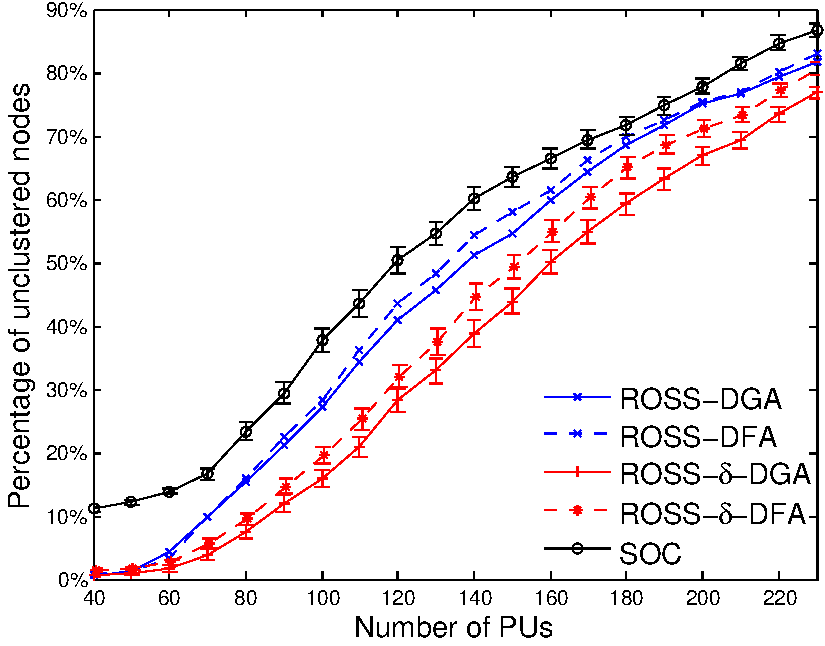
\includegraphics[width=\linewidth]{survival_rate_100_edge50.pdf}\par\caption{100 CRs}\label{singleton_clusters_100}
    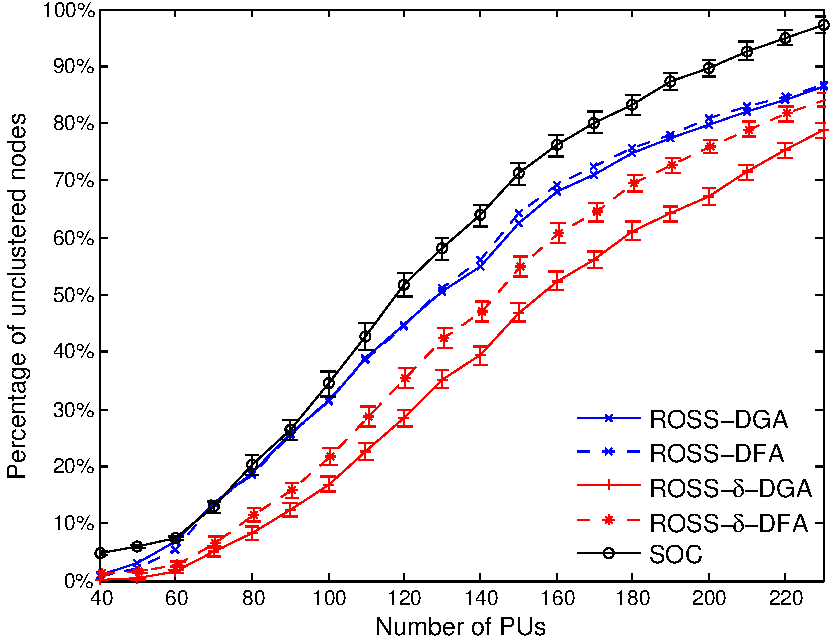
\includegraphics[width=\linewidth]{survival_rate_200_edge50.pdf}\par\caption{200 CRs}\label{singleton_clusters_200}
    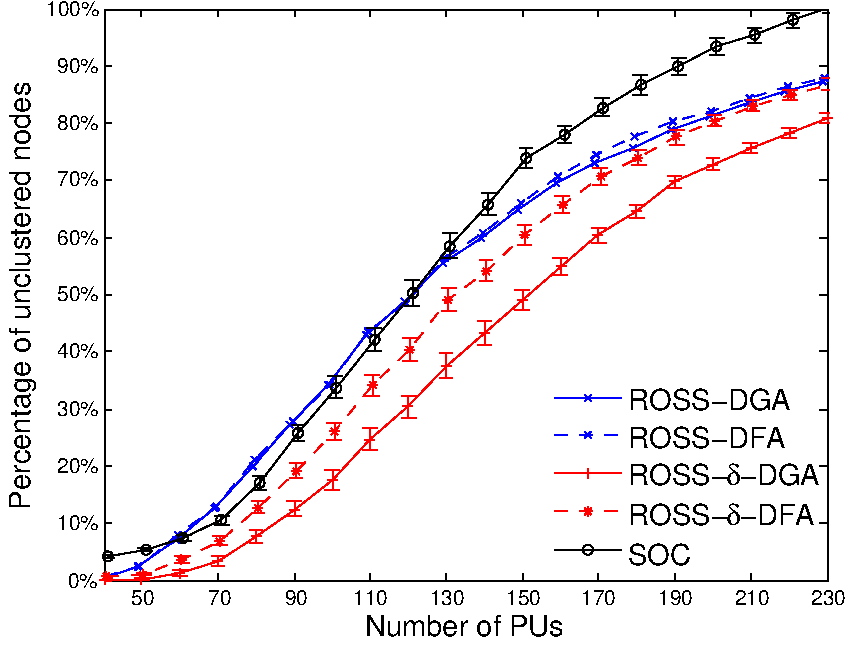
\includegraphics[width=\linewidth]{survival_rate_300_edge50.pdf}\par\caption{300 CRs}\label{singleton_clusters_300}
\end{multicols}
%\caption{Percentage of CR nodes which are not included in any non-singleton clusters}
%\label{unclustered_100_200_300}
\end{figure*}

%When the network is denser, the improvement on cluster sizes and robustness by the greedy search in the membership clarification phase is more obvious.

\begin{figure*}[t]
\begin{multicols}{3}
    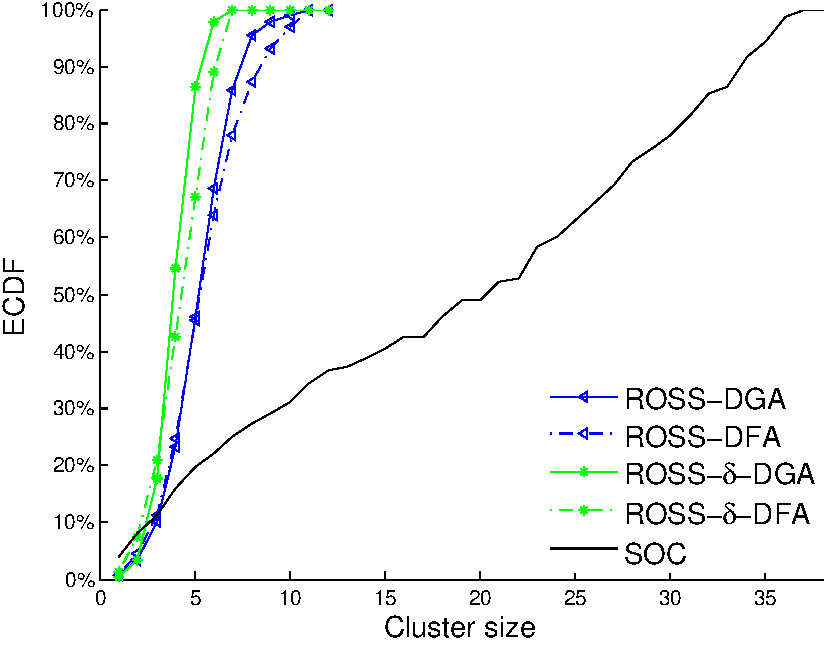
\includegraphics[width=\linewidth]{cdf_clusterSize_100.pdf}\par\caption{100 CRs, 30 PUs in network}\label{cdf_clusterSize_100}
    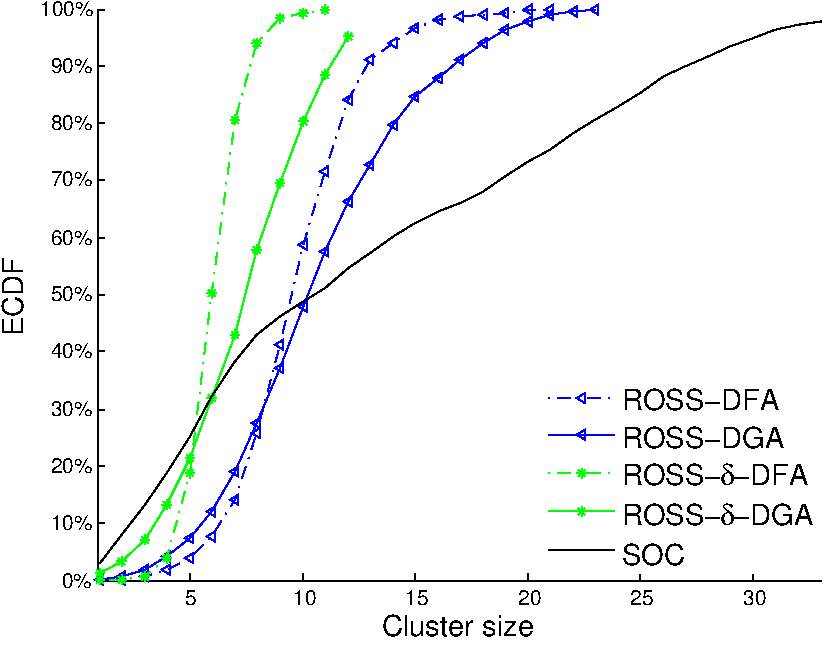
\includegraphics[width=\linewidth]{cdf_clusterSize_200.pdf}\par\caption{200 CRs, 30 PUs in network}\label{cdf_clusterSize_200}
    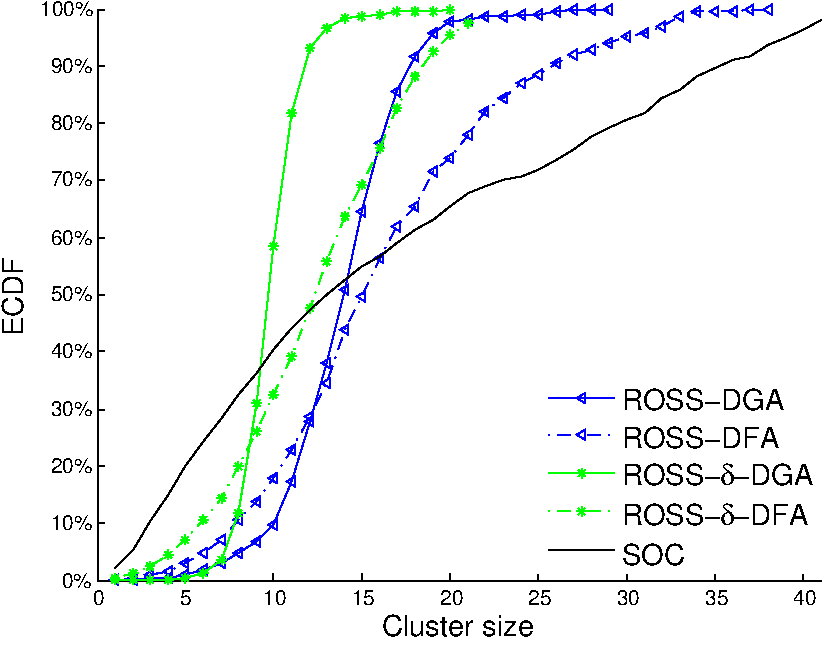
\includegraphics[width=\linewidth]{cdf_clusterSize_300.pdf}\par\caption{300 CRs, 30 PUs in network}\label{cdf_clusterSize_300}
\end{multicols}
%\caption{Cumulative distribution of CRs residing in clusters with different sizes}
%\label{cdf_100_200_300}
\end{figure*}

We next turn to the size of the formed clusters under the different distributed schemes.
For this we study in Figure~\ref{nClusters_largeNetwork} the average number of total clusters formed under the different schemes for the different parameter combinations considered.
The figure shows that the number of clusters resulting from SOC increases linearly, whereas the number of formed clusters increases sub-linearly in case of the variants of ROSS.
This result coincides with the analysis in Section~\ref{ross_p2_cluster_pruning}.
%When the network becomes denser, more clusters are generated by SOC compared with ROSS variants.
We furthermore consider the empirical distribution function of the size of the formed clusters, for each considered network density, in Figures~\ref{cdf_clusterSize_100}~\ref{cdf_clusterSize_200}~\ref{cdf_clusterSize_300} respectively.
\begin{figure}[!h]
  \centering
   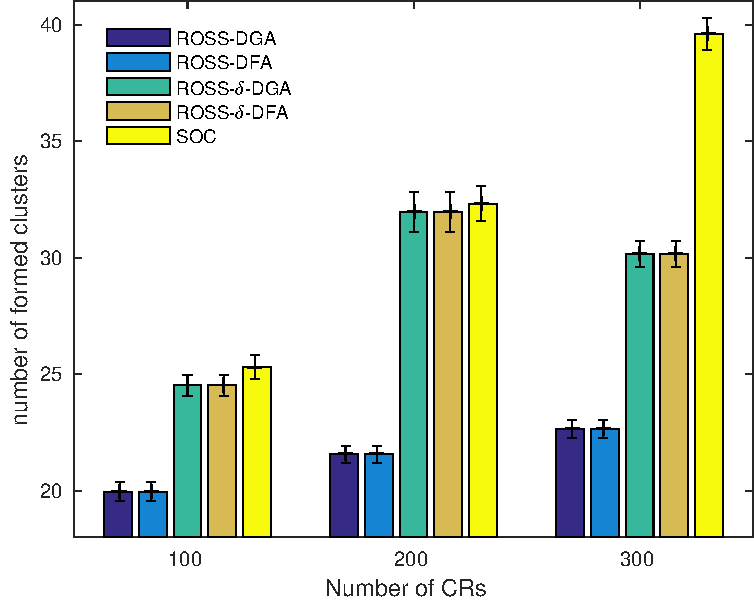
\includegraphics[width=0.7\linewidth]{nClusters_largeNetwork_no_texture.pdf}
  \caption{The number of formed clusters.}
  %, there are $x=6$ when $N=100$, $x=12$ when $N=200$, $x=21$ when $N=300$, which is around $2/3$ of the number of average neighbours.
  \label{nClusters_largeNetwork}
\end{figure}

The ECDF results show that the cluster sizes resulting from the variants of ROSS are clearly governed by the the desired size, \ie as shown in Figures~\ref{cdf_clusterSize_100}, 90\% of CR nodes are in clusters whose sizes are between 3 and 9, while for SOC, only 17\% of nodes are in the clusters with these sizes.
Similarly, when $N=200$ and the desired size is 12 (as shown in Figure~\ref{cdf_clusterSize_200}), 80\% of nodes are in clusters whose sizes are between 6 and 18, while only 30\% of nodes are in clusters of similar sizes when SOC is executed.
%Now we check how many CR nodes are in the clusters whose sizes deviate not much from the desired size, where we put the deviation limit at $\pm 50\%$ of the desired size.
The cluster sizes from ROSS-$\delta$-DGA and ROSS-$\delta$-DFA concentrate more around the desired size than that of ROSS-DGA and ROSS-DFA.

We finally turn to the results of clustering under erroneous spectrum sensing.
In Figure~\ref{false_negative_ccc} we first study the impact of erroneous spectrum sensing and subsequent clustering on the number of CCs per cluster.
The figure shows that the average number of CCs decreases slightly when the false negative rate increases.
Nevertheless, as with the previous investigated scenarios, the results do not show large differences between the distributed variants.
\begin{figure}[!h]
  \centering
   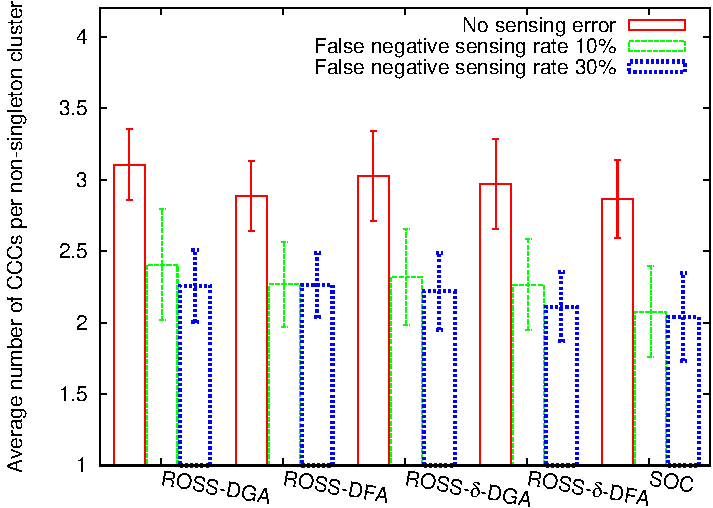
\includegraphics[width=0.7\linewidth]{false_negative.pdf}
  \caption{The number of CCs per non-singleton cluster with the presence of spectrum sensing false negative}
  \label{false_negative_ccc}
\end{figure}
We furthermore consider the ECDF of the size of the formed clusters under erroneous spectrum sensing in Figure~\ref{false_negative_CDF}.
For all the schemes, when the rate of false negatives increases, the number of singleton clusters and smaller clusters increases accordingly.
Clusters formed by SOC are furthermore affected by the sensing errors significantly.
More unclustered nodes are generated, and a lot of small clusters are formed, \eg when the false negative rate is 30\%.
In contrary, the ROSS variants are resilient in terms of unclustered nodes and cluster sizes.
We can conclude that due to the negotiation step within neighborhoods, ROSS variants successfully rule out the false negative channels resulting from erroneous spectrum sensing. 
This is an interesting and remarkabl advantage of ROSS in comparison to SOC.
\begin{figure}[!h]
  \centering
   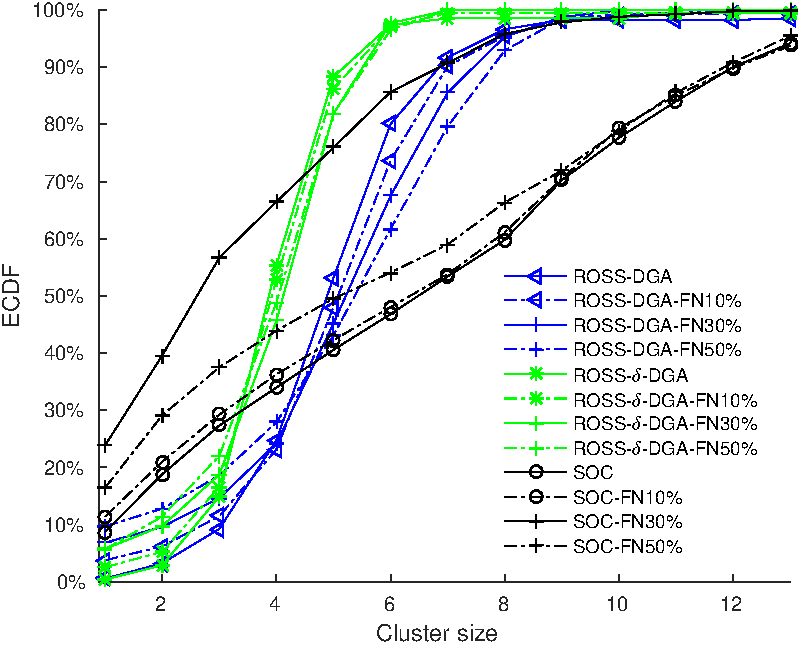
\includegraphics[width=0.7\linewidth]{draw_cdf_clusterSize_with_false_negative.pdf}
  \caption{100 CRs with false negative in spectrum sensing, 30 PUs in network}
  \label{false_negative_CDF}
\end{figure}

%\subsection{Discussion}
%Evaluating the small and the large scenarios lead to consistent insights.
%Firstly, our observations strengthen the claim that the average number of CCs per cluster is not necessarily a good metric to represent the robustness of a cluster.
%While ROSS and SOC have somewhat comparable results regarding the average size of the formed clusters, their robustness in case of additional primary user activity is strongly different.
%In contrast, for the centralized clustering scheme the claim is true that the number of CCs per cluster is a good measure for robustness.
%Furthermore, regarding the distributed schemes, the variants of ROSS outperform SOC considerably in the following four aspects.
%\begin{itemize}[noitemsep,topsep=0pt]
%\item The variants of ROSS result in less unclustered nodes than SOC for a given CRN, and the resulting clusters are more robust than the clusters formed by SOC.
%\item The amount of signaling overhead involved in ROSS is about half of that needed for SOC, and the signaling messages are much shorter that the latter.
%\item Compared with SOC, the clusters generated by ROSS don't appear with a wide span of sizes. ROSS with size control mechanism result in the clusters whose sizes are in proximity to the desired size.
%\item The variants of ROSS are more resilient against the erroneous spectrum sensing.
%\end{itemize}
%
%Moreover, the ROSS variants with size control features achieve similar performance to the centralized scheme in terms of cluster size, and the cluster robustness is similar when applying the variants of ROSS and the centralized scheme respectively.
%%
%Among the variants of ROSS, the greedy mechanism in ROSS-DGA helps to improve the performance on cluster size and cluster robustness at the cost of increased signaling overhead.
%%We also notice that as a metric, the number of CCs per non-singleton cluster doesn't indicate the robustness of clusters as shown in Figure~\ref{singleton_clusters} and \ref{unclustered_100_200_300}, although it is adopted as the metric in the formation of clusters.

\section{Conclusion}
\label{conclusion}
In this paper we investigate robust clustering problem in CRN thoroughly and propose both centralized and distributed clustering solutions.
We give mathematical description of the problem and prove NP hardness of it.
The proposed centralized scheme generate clusters which have long life expectancy against primary users, and the cluster sizes are close to the desired cluster size.
%The distributed scheme not only results in more robust clusters, but the cluster sizes are in a smaller range than the comparison scheme.
%The congestion game model in game theory is used to design the distributed schemes.
%A Light weighted clustering scheme ROSS is also proposed.
Through simulation, the distributed schemes demonstrate similar performance with the centralized scheme in terms of cluster robustness, signaling overhead and cluster sizes.
The distributed scheme outperforms the comparison distributed scheme by generating more robust clusters,  generating clusters whose sizes are in a smaller range, and being more resilient against the erroneous spectrum sensing.

% if have a single appendix:
%\appendix[Proof of the Zonklar Equations]
% or
%\appendix  % for no appendix heading
% do not use \section anymore after \appendix, only \section*
% is possibly needed

% use appendices with more than one appendix
% then use \section to start each appendix
% you must declare a \section before using any
% \subsection or using \label (\appendices by itself
% starts a section numbered zero.)
%

\vspace{50mm} %xx mm vertical space

\appendices
\section{Peudo Code for Algorithm~\ref{alg0}, \ref{alg_size_control_available_CCC}, \ref{alg4}}
\begin{algorithm}              % enter the algorithm environment
\caption{ROSS phase I: cluster head determination and initial cluster formation for CR node $i$}          % give the algorithm a caption
\label{alg0} 
\DontPrintSemicolon
\SetAlgoLined
\KwIn{$d_j, g_j, j\in \text{Nb}(i)\setminus \Lambda$, $\Lambda$ denotes the set of cluster heads among $\text{Nb}(i)$. Empty sets $\tau_1,\tau_2$}
\KwResult{Returning 1 means $i$ is cluster head, and $d_j$ is set to 0, $j\in \text{Nb}(i)\setminus \Lambda$. Returning 0 means $i$ is not cluster head.}
%C1-6-wording
\If{$\nexists j\in \text{Nb}(i)\setminus \Lambda$, such that $d_i \geq d_j$}{
	return 1;
	}
\eIf{$\exists j\in \text{Nb}(i)\setminus \Lambda$, such that $d_i > d_j$}{
	return 0;}{
	\If{$\nexists j\in \text{Nb}(i)\setminus \Lambda$, such that $d_j == d_i$}{
	$\tau_1 \leftarrow j$
	}
}
\If{$\nexists j\in \tau_1$, such that $g_i \leq g_j$}{
	return 1;
	}
\eIf{$\exists j\in \tau_1$, such that $g_i < g_j$}{
	return 0;
	}
	{\If{$\nexists j\in \tau_1$, such that $g_j == g_i$}{
		$\tau_2\leftarrow j$
		}
	}
\If{$\texttt{ID}_i$ is smaller than any $\texttt{ID}_j$, $j\in \tau_2\setminus i$}{
	return 1;
	}
	{return 0;
	}
\end{algorithm}


\begin{algorithm}               % enter the algorithm environment
\caption{ROSS phase I: cluster head guarantees the availability of CC (start from line 1) / cluster size control (start from line 2)}          % give the algorithm a caption
\label{alg_size_control_available_CCC}
\DontPrintSemicolon
\SetAlgoLined
\KwIn{Cluster C, empty sets $\tau_1, \tau_2$}
\KwOut{Cluster C has at least one CC, or satisfies the requirement on cluster size}
%\tcc*[r]{When to guarantee available CCs, execute from line 1, when to control cluster size, execute from line 2}
\While {$K_C =\emptyset$} {
\While{$|C|> t\cdot \delta$}{
	%calculate $\lambda = \min_{i\in C, i\neq H_C}(|K_{H_C}\cap K_i|)$;\\
	\eIf{$\exists$ only one $i\in C\setminus h(C)$, $i = \argmin(|K_{h(C)}\cap K_i|)$}{
			$C=C\setminus i$;
		}{
				$\exists$ multiple $i$ which satisfies $i = \argmin(|K_{h(C)}\cap K_i|)$;\\ $\tau_1\leftarrow i$;		
		}
		
	\eIf{$\exists$ only one $i\in \tau_1$, $i = \argmax(|\cap_{j\in C\setminus i} K_j|-|\cap_{j\in C} K_j|)$}{
		$C=C\setminus i$;
		}{
			%$\exists$ multiple $i$ which satisfies $i = \argmax(|\cap_{j\in C\setminus i} K_j|-|\cap_{j\in C} K_j|)$;\\
			$C=C\setminus i$, where $i = \argmin_{i\in \tau_1} \texttt{ID}_i $
			%$\texttt{ID}_i$ is smaller than any $\texttt{ID}_j$, $j\in \tau_2\setminus i$;
		}
	}
}
\end{algorithm}


%\section{}
\begin{algorithm}               % enter the algorithm environment
\caption{Debatable node $i$ decides its affiliation in phase II of ROSS}
%, chooses one claiming cluster to stay and leaves all the other claiming clusters}          % give the algorithm a caption,  cluster to settle
\label{alg4}
\DontPrintSemicolon
\SetAlgoLined
\KwIn{all claiming clusters $C\in S_i$}
\KwOut{one cluster $C\in S_i$, node $i$ notifies all its claiming clusters in $S_i$ about its affiliation decision.
}
\While{$i$ has not chosen the cluster, or $i$ has joined cluster $\tilde{C}$, but $\exists C'\in S_i, C'\neq \tilde{C}$, which has $|K(C'\setminus i)|-|K(C')|<|K(C\setminus i)|-|K(C)|$}{
	\eIf{$\exists$ only one $C\in S_i$, $C = \argmin(|K(C\setminus i)| - |K(C)|)$}{
			return $C$;
		}{
				$\exists$ multiple $C\in S_i$ which satisfies $C = \argmin(|K(C\setminus i)| - |K(C)|)$;\\ 
				$\tau_1\leftarrow C$;		
		}
	\eIf{$\exists$ only one $C\in \tau_1$, $C = \argmax(K_{h(C)}\cap K_i)$}{
			return $C$;
		}{
				$\exists$ multiple $C\in S_i$ which satisfies $C = \argmax(K_{h(C)}\cap K_i)$;\\ 
				$\tau_2\leftarrow C$;		
		}
	\eIf{$\exists$ only one $C\in \tau_2$, $C = \argmin|C|)$}{
			return $C$;
		}{
				return $\argmin_{C\in \tau_2}h(C)$;\\
		}
		}
\end{algorithm}


\section{Proof of Lemma~\ref{clustering:theorem}}
\begin{proof}
\label{proof_clustering:lemma1}
We consider a CRN which is represented by a connected graph.
% (COMMENT: Why is it necessarily connected? No special case where the graph has two components? ANSWER(Di): It is possible for the graph to have two components. My point it, when theorem works in one component, it works in the complete graph.)
To simplify the discussion, we assume that secondary users have unique individual connectivity degrees. 
Each user has an identical ID and a neighborhood connectivity degree.
This assumption is justified as the neighborhood connectivity degrees and node IDs are used to break ties in Algorithm~\ref{alg0}, when the individual connectivity degrees are unique, it is not necessary to use the former two metrics. 
%(COMMENT: What do you mean by breaking ties?? I don't see why your argument holds. ANSWER(DI): according to Algorithm 1, to decide whether node $i$ is a cluster head, the comparision on $i$'s certain degrees with its neighbors needs to be made. It is possible that $i$ has the same degree with some neighbors, then we need ID to decide whether $i$ is cluster head.)

%we assume every node has at least one neighbour.
For the sake of contradiction, let us assume there exist a secondary user $\alpha$ which is not included into any cluster.
Then there exists a node $\beta\in \text{Nb}(\alpha)$ such that $d_{\alpha} > d_{\beta}$ (otherwise $\alpha$ becomes cluster head). 
In this case, according to Algorithm~\ref{alg0}, $\beta$ is not included into any cluster, because otherwise $d_{\beta} = M$, a large positive integer, which contradicts to $d_{\alpha} > d_{\beta}$.
Now, we distinguish between two cases: 
%Otherwise, node $\alpha$ is eligible to form a cluster. COMMENT: unnecessary sentence!
If $\beta$ becomes cluster head, node $\alpha$ is included, the assumption is not true.
If $\beta$ is not a cluster head, then $\beta$ is not in any cluster, we can repeat the previous analysis made on node $\alpha$, and deduce that node $\beta$ has a neighboring node $\gamma$ with $d_{\gamma} < d_{\beta}$.
% (COMMENT: $\beta$ not being a cluster head and $\beta$ not belonging to any cluster is not the same statement!!! ANSWER(Di): I add some more words)
So far, when there is no cluster head identified, the unclustered nodes, \ie $\alpha$, $\beta$ form a linked list, where their connectivity degrees monotonically decrease.
But this list will not continue growing, because the minimum individual connectivity degree is zero, and the length of this list is upper-bounded by the total number of nodes in the CRN.
An example of the formed node series is shown as Figure~\ref{lemma1}.

\begin{figure}[ht!]
  \centering
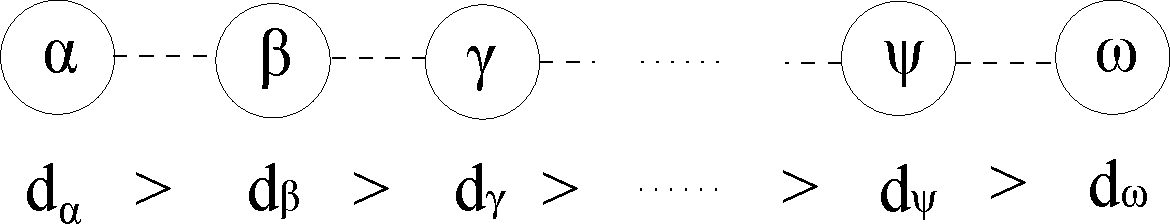
\includegraphics[width=0.6\linewidth]{lemma1.pdf}
% 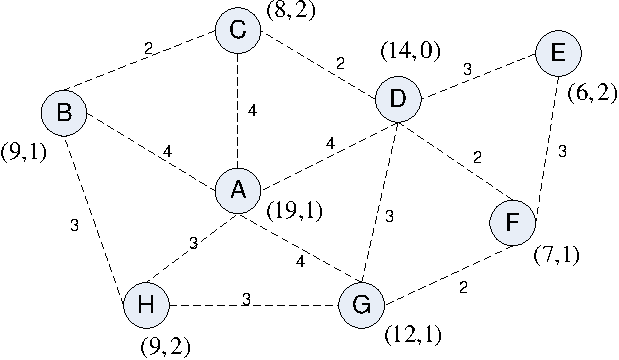
\includegraphics{figure1.pdf}
	\caption{The node series discussed in the proof of Theorem~\ref{clustering:theorem}, the deduction begins from node $\alpha$}
	\label{lemma1}
\end{figure}


In this example, node $\omega$ is at the tail of a list.
As $\omega$ does not have neighboring nodes with lower individual connectivity degree, $\omega$ becomes a cluster head.
Then $\omega$ incorporates all its one-hop neighbors (here we assume that every newly formed cluster has common channels), including the nodes which precede $\omega$ in the list.
The nodes which join a cluster set their individual connection degrees to $M$, which makes the node immediately precede in the list to become a cluster head.
In this way, cluster heads are generated from the tail to the head in the list, and every node in the list is in at least one cluster, which contradicts the assumption that $\alpha$ is not included in any cluster.

%If we see a secondary user \textit{becoming a cluster head}, or \textit{becoming a cluster member} as one step, as the length of the list of secondary users is not larger than $N$, there are $N$ steps for this scenario to form the initial clusters.

%we know that within at most $N$ steps, all the nodes belong to certain clusters. (XXXXXXX COMMENT: No, we don't! Where was that shown?)
\end{proof}


%
\section{Proof of Theorem~\ref{theorem1}}
\label{proof_theorem1}
\begin{proof}
To prove the robust clustering problem is NP-hard, we reduce the \textit{maximum weighted k-set packing problem}, which is NP-hard when $k\geqslant 3$~\cite{Computers_a_Intractability}, to the the robust clustering problem to show the latter is at least as hard as the former.
Given a collection of sets of cardinality at most $k$ and with weights for each set, the maximum weighted packing problem is that of finding a collection of disjoint sets of maximum total weight.
The decision version of the weighted $k$-set packing problem is,
\begin{mydef}
\label{def_kset_packing}
Given a finite set $\mathcal{G}$ of non-negative integers where $\mathcal{G} \subsetneq \mathbb{N}$, and a collection of sets $\mathcal{Q}=\{S_1,S_2,\cdots,S_m\}$ where $S_i \subseteq \mathcal{G}$ and $\max(|S_i|)\geq 3$ for $1 \leq i \leq m$.
Every set $S$ in $\mathcal{Q}$ has a weight $\omega(S) \in \mathbb{N}^+$. 
%
The problem is to find a collection $\mathcal{I} \subseteq \mathcal{Q}$ such that $\mathcal{I}$ contains only the pairwise disjoint sets and the total weight of these sets is greater than a given positive number $\lambda$, i.e., $\sum_{\forall S \in \mathcal{I}} \omega(S) > \lambda$.
\end{mydef}


%First, we argue that robust clustering problem is in NP, since given a collection of clusters, a certifier can efficiently check that such clusters are pairwise disjoint, indeed contains all the CR nodes in the CRN $\mathcal{N}$ and the sum of $f(C)$ as shown in Definition~\ref{def_centralized_clustering} is greater than a certain value.

We will show that the weighted $k$-set packing problem $\leq_P$ CRN robust clustering problem.
Given an instance of the weighted $k$-set packing problem, \ie a collection of sets $\mathcal{Q}=\{S_1,S_2,\cdots,S_m\}$, where the set $S_i, i\in \{1,2,\ldots,m\}$ consists of positive integers.
There is an integer weight $\omega(S_i)$ for $S_i$, in the end an integer $\lambda$ completes the description of this instance.
We will construct an instance of a CRN robust clustering problem within polynomial time.
W.l.o.g. we let set $\cup_{i\in\{1, 2,\ldots, m\}}S_i = \{ 1, 2,\ldots , N \} = \mathcal{P}$.

We will construct the CRN and the clusters as follows:
For every set $S\in \mathcal{Q}$, there will be a corresponding cluster composed with CR nodes constructed.
For the set whose size is larger than 1, the IDs of the constructed CR nodes are identical with the elements in it, and we locate the CR nodes so that any two of them can communicate directly when common channels are available on them.
Besides, a set of channels with cardinality of $|\omega(S)|$ is allocated to all the CR nodes in this cluster, and the channels are on the spectrum band which is exclusive for this cluster.
For the set $S$ which contains only one element, \ie $S =\{t\}$ where $t\in\mathcal{P}$, a cluster composed with two CR nodes will be created.
In this case, one CR node's ID is $t$, the other CR node is the dummy node of the former and its ID is $t+N$.
A number of $|\omega(S)|$ channels from the exclusive spectrum band for this cluster are allocated to these two CR nodes.
Now we have constructed the clusters which correspond to all the sets in $\mathcal{Q}$.
Note that every CR node is allowed to form a singleton cluster by itself, although its common channels don't contribute to the sum of $f(C)$.
%In the end, we construct the singleton clusters, \ie for each element in $\mathcal{P}$, a corresponding singleton cluster is constructed.
%In particular, if the CR node has been constructed and has been in certain clusters already through the previous steps, the CR node with all the channels assigned to it constitute a singleton cluster.
%If there is an element in $\mathcal{P}$, which doesn't has a corresponding CR node yet, we simply construct this singleton cluster by adding that CR node, and assign it with a random number of channels from a exclusive spectrum band.
%We call the latter kind of clusters the \textit{auxiliary singleton clusters}.

Actually, all the constructed CR nodes can be assumed to locate in a very small area so that each CR node is within the transmission scope of every other CR node.
Note that in each constructed cluster, the CR nodes occupy the common channels which are exclusive to this cluster, this design of transformation eliminates the formation of the cluster which doesn't have a corresponding set in $\mathcal{Q}$.
The existence of the singleton clusters ensures that it is always possible to find out a group of clusters, which together constitute the whole CRN.
%Now we have completed a CRN and can claim that all the constructed clusters $C$ constitute the complete CRN network $\mathcal{N}$.

Now suppose there is a set of pairwise disjoint clusters which constitute the CRN $\mathcal{N}$, and the sum of $f(C)$ is greater than $\lambda$.
After removing the singleton clusters, we can easily find the natural association between the remaining clusters and the sets in $\mathcal{Q}$. 
The clusters in the CRN correspond to the sets in $\mathcal{Q}$ according to the mapping between the node IDs in the clusters and the elements in the sets.
In particular, the clusters which contain dummy CR nodes correspond to the sets which contain only one element.
Then the sum of the weights of the corresponding sets equals to the sum of $f(C)$ and thus greater than $\lambda$.




We have now shown that our algorithm solves the weighted $k$-set packing problem using a black box for the robust clustering problem. 
Since our construction takes polynomial time, we can conclude that the robust clustering problem is NP-hard.
%\begin{itemize}
%\item First, all the sets in the instance $\mathcal{I}$ are mapped sequentially to a group of clusters, \ie for a set $S\in\mathcal{I}$, the elements in $S$ are mapped to CR nodes which compose a cluster $C$, moreover, the resultant CR node's ID equals to the corresponding element in $\mathcal{S}$.
%This transformation takes $N$ steps.
%\item If $\mathcal{I}$ is not the solution because the intersection of two sets is not empty, the resultant clusters are not the solution to the clustering problem due to the overlapped clusters.
%When $\mathcal{I}$ contains only the disjoint sets, for each mapped cluster $C$, we assign the available channels for the nodes in $C$ so that the number of common channels in $C$ equals to the weight $\omega(S)$.
%This step of transformation takes $N*|\mathcal{K}|$ steps where $\mathcal{K}$ is the set of licensed channels.
%\item The resultant clusters are not an instance for the robust clustering problem yet because the clusters don't include all the CR nodes in the CRN, just as the instance $\mathcal{I}$ doesn't include all the elements in $\mathcal{G}$.
%We add the CR nodes besides the mapped clusters, which correspond to the elements in $\mathcal{G}\backslash\mathcal{I}$.
%We can randomly assign available channels on these newly added CR nodes, which do not contribute to the sum of the numbers of the common channels $f(C)$ as defined in~\ref{def_centralized_clustering} because they actually form singleton clusters and their cluster sizes are smaller than 2.
%This steps takes at most $N$ steps.
%
%
%\end{itemize}
%In this way, we change any instance of a weighted $k$-set packing problem into an instance of robust clustering.
%%The polynomial algorithm $\sigma$ consists of three steps.
%%\begin{itemize}
%%
%%\item First, the sets in the instance $\mathcal{I}$ are mapped sequentially to the clusters of CR nodes on a two-dimensional Euclidean plane, where the CR user ID is identical with the corresponding element's index.
%%
%%\item Second, for each mapped cluster $C$, we assign the channels for the nodes in $C$ so that $|K(C)|$ equals to the $\omega(S)$.
%%We can simply assign the first $|K(C)|$ channels to each CR node in $C$, without considering the possible mismatch when the same CR node appears in different clusters and is assigned with different channels.
%%
%%\end{itemize}
%%The number of steps is dependent on $\mathcal{I}$, which is between 1 and $N^2$.
%%
%Assume we have a robust clustering black box which checks whether the clustering instance meets the requirement, \ie clusters are not overlapping, and the sum of CCs of the clusters whose size is larger than 1 exceeds $\lambda$ or not.
%\begin{itemize}
%\item If \textit{yes} is said, then the total weight of the corresponding instance of the maximum weighted k-set packing problem is greater than $\lambda$.
%\item If the black box says \textit{no}, either due to overlapping clusters or the sum of CCs is smaller than $\lambda$, the corresponding instance of the packing problem is not a solution.
%\end{itemize}
%
%
%
%% The direction is wrong!!
%%When $\mathcal{I}$ is not an instance for weighted $k$-set packing problem due to the existence of joint sets, the corresponding clustering instance is not a successful cluster partition for the robust clustering problem, as there are overlapped clusters.
%%%
%%When the sets in an instance $\mathcal{I}$ for weighted $k$-set packing are disjoint, the sum of weights is identical to the total number of the CCs in the CRN which are mapped from $\mathcal{I'}$.
%%Thus, when a instance $\mathcal{I}$ for $k$-set packing problem is true (or false), \ie the sum of weights is greater than $\lambda$, then in the CRN which is mapped from $\mathcal{I'}$, the sum of the numbers of CCs of the clusters is greater (or smaller) than $\lambda$.
%
%Hence, the weighted $k$-set packing can be reduced to the robust clustering problem in CRN, thus the latter problem is as hard as the former thus is of NP-hard.
%%An example of the reduction is shown in Table~\ref{no_hard_proof_instance}.



\end{proof}



\bibliographystyle{IEEEtran}
\bibliography{../backmatter/myrefs}


%\ack This class file was developed by Sunrise Setting Ltd,
%Paignton, Devon, UK. Website:\\
%\href{http://www.sunrise-setting.co.uk}{\texttt{www.sunrise-setting.co.uk}}


\end{document}
